\section{Topological Spaces}

% Briefly, I will present the basic concepts of the field of topology.
% While we don't later deal with topological matters in the core of this thesis, the construction of manifolds is a topological topic that we later add additional notions to in order to arrive at one of the main topics of study in this thesis, Riemannian manifolds.
% It makes sense therefore to present this separately, to make clear the delineation between topological manifolds, and what concepts come from this part of mathematics, and what additional stucture is gained by additional imposing the Riemannian metric that take maifolds from being topological to Riemannian.

Intuitively, the study of topology is the study of spaces that we identify as the same if we can "continuously" deform one into another - as if the space is made of rubber that can be stretched and deformed.
Another way to think about it is the weakening of the structure of a \emphmarginnote{metric space} that allows us to extend certain tools to new spaces.
It allows us to discuss whether points are "near" each other without needing to being able to say how far apart exactly they are.

\begin{definition}[Metric space]
	A metric space \((X, d)\) is a space \(X\) with a two argument function \(d: X\times X \to \R_{\geq 0}\) such that \(d\) satisfies:
	\1 \(d(x, x) = 0\) for \(x\in X\).
	\2 If \(x \neq y\) for \(x, y\in X\) then \(d(x, y) > 0\) (Positivity)
	\3 \(d(x, y) = d(y, x)\) for \(x, y \in X\) (Symmetry)
	\4 \(d(x, z) \leq d(x, y) + d(y, z)\) for \(x, y, z \in X\) (Triangle inequality)
	\0
\end{definition}
This encodes in its structure our intuitive notion of a \emphmarginnote{distance function} in \(d\) between points in the space \(X\).
On top of this we can create two notions.

First is that of \emphmarginnote{open sets}. 

\todo[inline]{Consider this intro via metric spaces - I think it is more intuitive but we shall wsee. Discuss w valentin}

One motivation behind the modern definition of a topology comes from the "open set criterion", the observation that continuous functions between metric spaces (defined in the \(\del{\epsilon, \delta}\) sense \todo{cite?
}) can be defined by knowing only the open sets of the metric spaces and throwing out the metrics that generated the open sets in the first place.
\begin{definition}[Topology]
	A topological space \((X, \topo{X})\) is a set \(X\) along with a collection of subsets \(\topo{X}\) of \(X\), called the \emphmarginnote{open sets} of \(X\) that satisfy the following:
	\begin{itemize}
		\item \(X\) and \(\emptyset\) are elements of \(\topo{X}\).
		\item \(\topo{X}\) is closed under \emph{finite} intersections.
		\item \(\topo{X}\) is closed under \emph{arbitrary} unions.
	\end{itemize}
\end{definition}
A point in a topological space can be said to be "near" another is it is in a \emphmarginnote{neighbourhood} of the point.
A neighbourhood of \(x \in X\) is simply an open set containing \(x\).
The neighbourhood of a set \(S\subset X\) is an open set containing \(S\).

This definition of a topology takes open sets as the primary element.
Relatedly of importance are \emphmarginnote{closed sets}.
A set in a topology is closed if its compliment in \(X\), \(X \backslash S\) is open.
Note despite the name, these properties are not opposite.
Sets can be neither, just closed, just open, or both.
In all topologies \(X\) and \(\emptyset\) are both open and closed.
A topology can just as well be defined by its closed sets, but by convention we specify the open ones.

On any given space we can define many topologies, although only some are useful.
We say that a topology is \emph{coarser} than another if it is a subset of the other topology.
Conversely, a topology that contains another topology is said to be \emph{finer} than that topology.

The \emphmarginnote{interior} of a set \(S\), \(\inte S\) is the union of all open sets in \(\topo{X}\) contained in \(S\).
The interior of any set is open.
\\
The \emphmarginnote{exterior} of a set \(S\), \(\ext S\), is the union of all open sets in \(\topo{X}\) contained in \(X \backslash S\).
The exterior of any set is open.
\\
The \emphmarginnote{closure} of a set \(S\), \(\closure{S}\), is the intersection of all closed set in \(\topo{X}\) containing \(S\).
The closure of any set is closed.
\\
The \emphmarginnote{boundary} of a set \(S\), \(\boundary S\), is the set of all points not in \(\inte S\) or \(\ext S\).
The boundary of any set is a closed set.
\\
A point \(p\in S\) is said to be \emphmarginnote{isolated} in \(S\) if \(p\) has a neighbourhood in \(\topo{X}\) such that \(U \^ S = \cbr{p}\).\\
A point \(p\in X\) (not \(S\)) is said to be a \emphmarginnote{limit point} of \(S\) if every neighbourhood of \(p\) contains a point in \(S\) that is not \(p\).
Topologically closed sets contain all such limit points within themselves.
\\
A set \(S\) is said to be \emphmarginnote{dense} in another set \(T\) if \(\closure{S} = T\).
A classic example is that the rational numbers \(\Q\) are dense in the reals \(\R\).

\begin{figure}[h]
	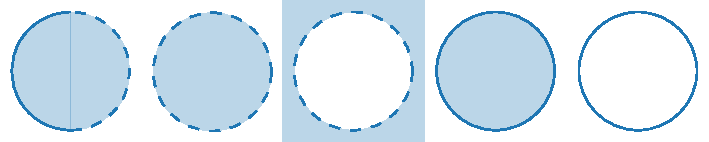
\includegraphics{figures/diagrams/set_properties.pdf}
	\caption{From left to right: \(S\), \(\inte S\), \(\ext S\), \(\closure{S}\), \(\boundary S\).}
\end{figure}

\subsection{Continuity \& Convergence}

The two most important notions in topology are those of \emph{continuous functions} and \emph{sequential convergence}.

% A topology allows us to discuss a series notions commonly discussed in relation to metric spaces without that additional structure. Some of these are \textit{locality, convergence, continuity, compactness, paracompactness, denseness}, along with a others.

% A property of a topological space is said to hold \emphmarginnote{locally} if it is true for one of the following two cases:
% \1 Each point has a neighbourhood exhibiting the property.
% \2 Each point has a neighbourhood basis of sets exhibiting the property
% \0
% Condition 2 is much stronger than condition 1.

Continuous functions between two topological spaces preserve in one direction only the structure of the topology of the two spaces.
% \begin{definition}[Continuous functions]
%     A function \(f: X\to Y\) between two topological spaces \(\del{X, \topo{X}}\) and \(\del{Y, \topo{Y}}\) is said to be continuous if for every open set \( V \in \topo{Y}\), its preimage is open in \(X\), \(f^{-1}(V) \in \topo{X}\).
% \end{definition}
\todo[inline]{consider the more formal defnition based style vs the text based style}
% A function \(f: X\to Y\) between two topological spaces \(\del{X, \topo{X}}\) and \(\del{Y, \topo{Y}}\) is said to be \emphmarginnote{continuous} if for every open set \( V \in \topo{Y}\), its preimage is open in \(X\), \(f^{-1}(V) \in \topo{X}\).
\begin{definition}[Topological continuity]
	A function \(f: X\to Y\) between two topological spaces \(\del{X, \topo{X}}\) and \(\del{Y, \topo{Y}}\) is \emph{continuous} if for every open set \( V \in \topo{Y}\), its preimage is open in \(X\), \(f^{-1}(V) \in \topo{X}\).
\end{definition}
\begin{figure}[h]
	
\includegraphics{figures/tex/continuous.tex}
\end{figure}
Compositions of continuous functions are continuous, and so are their restrictions to open sets.
Continuity can be proved by proving continuity just for a basis on \(\topo{Y}\).

If a bijective function and its inverse are both continuous, then that function is said to be a \emphmarginnote{homeomorphism}, as it preserve the topological structure of the two spaces.
If there exists a homeomorphism between \(X\) and \(Y\) then we say that \(X\) and \(Y\) are \emphmarginnote{homeomorphic}, denoted \(X \isomtop Y\) (isomorphic in the topological sense).

A weaker but important notion is that of a \emphmarginnote{local homeomorphism}.
A function \(f\) is a local homeomorphism if for every point \(x\in X\) has a neighbourhood \(U\) such that the restriction of \(f\) to \(U\), \(\eval{f}_U\), is a homeomorphism from \(U\) to \(f(U)\).
If there exists a local homeomorphism between \(X\) and \(Y\) then we say they are \emphmarginnote{locally homeomorphic}.

Convergence in the topological sense implies a sequence becomes arbitrarily close to a point in the sense of neighbourhoods of the point.
% \begin{definition}[Convergence]
%     The point \( x \in X \) is said to be the limit of a sequence \(\cbr{x_i}_{i=0}^\infty\) if for every neighbourhood \(U\) of \( x \), there is and \(N_U \in \N\) such that for all \( i > N_U \), \( x_i \in U\).
% \end{definition}
The point \( x \in X \) is said to be the \emphmarginnote{limit of a sequence} \(\cbr{x_i}_{i=0}^\infty\) if for every neighbourhood \(U\) of \( x \), there is and \(N_U \in \N\) such that for all \( i > N_U \), \( x_i \in U\).
Alternatively we might say that \(\cbr{x_i}_{i=0}^\infty\) \emphmarginnote{converges} to \(x\), denoted \(\cbr{x_i}_{i=0}^\infty x\) or even \(x_i \to x\) for short.
\begin{figure}[h]
	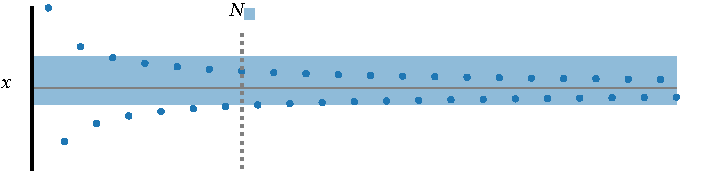
\includegraphics{figures/diagrams/neighbourhood.pdf}
	\caption{The sequence \(\cbr{
\includegraphics{figures/diagrams/tab_blue_scatter.pdf}_i}\) converges to the point \(x\).
		We see that on the neighbourhood \bluesquare{}, for \(i > N_{\bluesquare{}}\), \(
\includegraphics{figures/diagrams/tab_blue_scatter.pdf}_i \in \bluesquare{}\)} \end{figure} 
\todo{figure the symbols better}
A set \(S\) is is said to be \emphmarginnote{sequentially closed} if it contains the limits of all sequences in \(S\).
% abc123def
This notion is \emph{different} ot that of \emph{topologically closed} introduced earlier, and is different to the notion of containing all of its \emph{topological limit points}.
Topological closure implies sequential closure, but not the converse.

A useful combination of these notions is the convergence of sequences under continuous maps.
If a sequence \(x_i \to x\), and we have \(f: X\to Y\) continuous, then \(f(x_i) \to f(x)\).

\subsection{"Goldilocks" topologies}
The definition of a topology along with the notions we have introduced can sometimes lead to paradoxical results.
On one end if we endow \(X\) with the topology with the least sets, the \emphmarginnote{trivial topology}, \(\topo{X} = \cbr{X, \emptyset}\), then every sequence converges to every point in \(X\).
By contrast if we endow \(X\) with the \emphmarginnote{discrete topology}, the topology that defines \emph{every} subset of \(X\) as open, then it is \emph{totally disconnected}, i.e. that every point is completely separated from every other point.
In order to avoid these pathologies in "nice" spaces, we introduce a some more notions so that our topologies have the right amount of open sets to be useful to us.

A \emphmarginnote{Hausdorff space\label{def:hausdorff}} ensures that we have \emph{enough} open sets in our topology.
A space is said to be Hausdorff if for any two points \(x_1, x_2 \in X\), we can find two open sets \(U_1, U_2\) such that \(x_1 \in U_1\), \(x_2 \in U_2\), but \(U_1 \cap U_2 = \emptyset\).
Intuitively this says if I have any two points, I can always separate them into two distinct neighbourhoods.
Being a {Hausdorff space} implies two very useful properties: \1 Every 1-point set \(\cbr{x}\) is closed.
\2 If a sequence \(\cbr{x_i}\) in \(X\) converges to a limit \(x\), then this limit is \emph{unique}.
\0
On a finite set, only the discrete topology is Hausdorff.
On infinite sets, many might be.
The Hausdorff property is not the only possible "separability" criteria, it exists in a scale of strictness, but it is the most useful to us.

Secondly we have the notion of \emphmarginnote{countability}.
This ensures we don't have \emph{too many} open sets in our topology.
To introduce this, we first introduce the notion of a \emph{basis} of a topology.

A topology can often be constructed by specifying some special set of open sets, and "completing" this in a suitable manner.
% \begin{definition}[Basis]
%     A basis \(\c{B}\) of \(X\) is a collection of subsets such that their union is \(X\), and for all \(B_1, B_2 \in \c{B}\), there is a \(B_3 \in \c{B}\) such that \(B_3 \subset B_1 \cap B_2\)
% \end{definition}
A \emphmarginnote{basis} \(\c{B}\) of \(X\) is a collection of subsets such that their union is \(X\), and for all \(B_1, B_2 \in \c{B}\), there is a \(B_3 \in \c{B}\) such that \(B_3 \subset B_1 \cap B_2\).

A basis can be completed into a topology by adding to it all possible unions of the sets in the basis.
This topology is said to be \emph{generated} by the basis.
Bases are useful as they give us something \emph{simpler} from which we can reconstruct the whole topology.

In some sense opposite, we have the notion of a \emphmarginnote{neighbourhood basis}.
If we consider \emph{all} the neighbourhoods of a point or set, \(\c{N}(x)\), then a neighbourhood basis \(\c{B}\) is a subset of \(c{N}(x)\) such that for any neighbourhood \(U \in \c{N}(x)\) there is an element in the neighbourhood basis \(V \in \c{B}\) such that \( V \subset U\).
This says that for any neighbourhood we can find a set in the neighbourhood basis that is contained within it.
This is useful as it allows us to study properties only "very close" to the point, forgetting about the rest of the topology.

In the discrete topology, the set \(\cbrcolon{\cbr{x}}{x\in X}\) is a basis and the set \(\cbr{x}\) is a neighbourhood basis of \(x\) as all points are separated from each other.

A space is \emphmarginnote{first-countable} if every point has a countable neighbourhood basis.
First countability implications regarding \emph{sequential closure} and \emph{topological closure}.
Previously we had that topological closure \(\implies\) sequential closure, but topological closure \(\centernot\implies\) sequential closure.
First countability results in topological closure \(\iff\) sequential closure, i.e. the topological and sequential notions of closure become identical.
Every metric space is first countable, but not necessarily the converse.

A space is \emphmarginnote{second-countable} if its topology has a countable basis.
Second countability implies first countability, as it must contain a countable neighbourhood basis for each point.

This condition is often used to reduce the number of sets on needs to "cover" a space \(X\).
A collection of subsets \(\c{U}\) is called a \emphmarginnote{cover} of \(X\) if for every point in \(X\), there is a \(U \in \c{U}\) such that \(x \in U\).
An \emphmarginnote{open cover} is a cover where all the subsets are open.
A \emphmarginnote{subcover} is a subset of a cover that remains still a cover.
In a second countable space, every open cover of the space has a \emph{countable} subcover.

% Most reasonable spaces we deal with are Hausdorff and second countable. Importantly these properties both hold of Euclidean space. For any two points \(x_1, x_2\) in \(\R^n\) separated by distance \(r\), the open ball neighbourhoods \(B_{\bar{r}}(x_1), B_{\bar{r}}(x_2)\), \(\bar{r} < r/2 \), and so it is Hausdorff. The topology can be generated by the basis of open balls \(\c{B} = \cbrcolon{B_r(x)}{r \text{ is rational and } x \text{ has rational coordinates}}\)

\subsection{Constructing topologies}

Many import spaces can be constructed out of other spaces.
When doing this we need to define the topology on these new spaces.
4 examples of particular importance are: \emph{subspaces}, \emph{products}, \emph{disjoint unions} and \emph{quotients}.
We will choose canonical ways to define these new topologies that preserve sensible properties on the new spaces.

\subsubsection{Subspaces}
\label{sec:topo_subspaces}

If we have \(S \subseteq X\), then the \emphmarginnote{subset topology} is the topology \(\topo{S} = \cbrcolon{U \^ S}{U \in \topo{X}} = S \^ \topo{X}\), i.e the intersection of the topology of \(X\) with \(S\).
We define the \emphmarginnote{inclusion map} \(\inclusion_S: S \hookrightarrow X\) as the restriction of the identity of \(X\) to \(S\), \(\eval{\id}_S\).

A continuous, \emph{injective} map \(f: X\to Y\) is called a \emphmarginnote{topological embedding} if it is a homeomorphism onto its image in \(Y\), \(f(X) \subseteq Y\), endowed with the subspace topology.

This definition is motivated by the \emphmarginnote{characteristic property of the subset topology}: if \(Y\) is a topological space, \(f: Y \to S\) is continuous if and only if the composition \[Y\xrightarrow{f}S\xhookrightarrow{\inclusion_S}X \] is continuous.
The subset topology is the unique topology satisfying this property.
% \(\inclusion_S\circ f: Y \to X\)

This induces a number of properties with respect to \(\topo{X}\) and the subset topology on \(S\), \(S\^ \topo{X}\): \begin{enumerate}[noitemsep] \item The inclusion map is a topological embedding.
	\item The closed subsets of \(S\) are the intersection of the closed subsets of \(X\) with \(S\).
	\item If \(f: X \to Y\) is continuous, then \(\eval{f}_S: S \to Y\) is continuous.
	\item If \(\basis\) is a basis of \(X\), then \(\basis_S = \cbrcolon{B\^S}{B \in \basis}\) is a basis of \(S\).
	\item If we have \(T \subset S \subset X\) then the topology \(T\^ \del{S\^ \topo{X}}\) agrees with \(T\^ \topo{X}\).
	\item If \(X\) is Hausdorff, then \(S\) is Hausdorff.
	\item If \(X\) is first countable, then \(S\) is first countable.
	\item If \(X\) is second countable, then \(S\) is second countable.
\end{enumerate}
The converse of 3.
allows us to show that \emphmarginnote{continuity is local}.
If we have \(f: X\to Y\), and for every point \(x\in X\) we have a neighbourhood \(U\) such that \(\eval{f}_U\) is continuous, then \(f\) is continuous.

Alternatively, we can \emphmarginnote{glue continues maps} together.
If we have a) \(B_1,.
..,B_n\), a finite collection of closed sets or b) \(\cbr{B_i}_{i\in A}\), any collection of open sets such that \(\u_{a\in A}
B_a = X\), and a continuous function for each \(B\), \(f_i: B_i \to Y\), and these functions agree on intersections, \(f_i(B_i \^ B_j) = f_j(B_i \^ B_j)\), then there is a unique continuous function \(f: X\to Y\) such that \(\eval{f}_{B_i} = f_i\).
A important corollary of this is that to check continuity it is sufficient to check continuity on a basis of \(X\).

\subsubsection{Product spaces}

Now consider the product of a finite collection of spaces \(X_1, .
.., X_n\).
Define a basis by \[\basis = \cbrcolon{U_1 \times .
		.. \times U_n}{U_i \in \topo{X_i}, i=1,..,n}\], the Cartesian product of each combination of sets from each topology.
The topology generated by this basis is the \emphmarginnote{product topology}.

The \emphmarginnote{characteristic property of the product topology} is that, for any topological space \(Y\), \(f: B\to X_1\times .
..
X_n\) is continuous if and only if the composition with each projection function \(\pi_i: x_1, .
.., x_n \mapsto x_i\), \(f_i = \pi_i \circ f\) is continuous.
The product topology is the unique topology for which this holds.

This induces a number of properties with respect to product topology on \(X_1\times.
.. \times X_n\):
\begin{enumerate}[noitemsep]
	\item Each projection map \(\pi_i\) is continuous.
	\item For continuous functions \(f_i: X_i \to Y_i\), the \emphmarginnote{product map} \(f_1 \times ... \times f_n: X_1 \times .. \times X_n \to Y_1\times ... \times Y_n\), \(f(x_1, ..., x_n) = (x_1, ..., x_n)\) is continuous.
	\item If we have subspaces \(S_i \subseteq X_i\), then the product topology \(S_1\^\topo{X_1} \times ... \times S_n\^\topo{X_n}\) coincides with the subspace topology \((S_1\times ... \times S_n) \^ \topo{X_1 \times ... \times X_n}\).
	\item For any \(i\), and picking \(a_j \in X_j, i\neq j\), then the map \(x \mapsto (a_1, ..., x, ..., a_n)\) it a topological embedding into the product space \(X_1 \times ... \times X_n\).
	\item If \(\basis_i\) is a basis for each \(X_i\), then \(\basis \cbrcolon{B_1 \times ... \times B_n}{B_i\in \basis_i}\) is a basis of \(X_1 \times ... \times X_n\).
	\item Every finite product of Hausdorff spaces is Hausdorff.
	\item Every finite product of first countable spaces is first countable.
	\item Every finite product of second countable spaces is second countable.
\end{enumerate}

For products of an infinite collection of spaces, a piece of subtly creeps in.
We want all the properties above to continue to hold.
But, as it turns out the basis we defined earlier is not a good choice.
On infinite spaces this is known as the \emphmarginnote{box topology}, where we take the products of all the open sets of each space.
This topology fails in a number of ways.
The box topology fails to preserve compactness through products.
For example, functions we expect to be continuous fail to be continuous, and topological convergence becomes a significantly strict condition under the box topology.

Instead we introduce the concept of \emphmarginnote{cylinder sets}.
For collection of spaces, each with a collection of subsets, \((X_a, \c{S}_a)_{a\in A}\), we take the Cartesian product of these to give \(X = \prod_{a\in A}\).
We get a canonical projection for each \(a\), \(\pi_a: X_a \to X\), that elements of \(X_a\) to its component in \(X\).
A \emph{cylinder set} is then a set \[\Int_{i=1}^n \pi_{a_i}^{-1}(S_{a_i}), \quad\quad S_{a_i} \in \c{S}_{a_i}, a_i \in A \].
Note this is a \emph{finite} intersection.
Alternatively we can see the cylinder sets as \[\cbrcolon{U_1 \times U_2 \times .
		..}{U_i \in \topo{X_i}, i=1,2,..., U_i \neq X_i \text{ for finitely many } i} \label{eq:cylendar_sets}\], products of subsets of each \(X_a\) where only \emph{finitely many} of the subsets are not the whole space \(X_a\).

We then define the \emphmarginnote{product topology on infinite products} to be the one generated by the basis of cylinder sets on the product of \((X_a, \topo{X_a})_{a\in A}\).
This topology is the one compatible with the previously stated conditions, and is the default topology on infinite products.
In the product topology, topological convergence coincides with the notion of \emphmarginnote{pointwise convergence}, i.e. a sequence of functions converge if and only if each of the component functions \(f_i\) converge.

On finite products, we can see that these two definitions coincide, and so we can use the cylinder sets to define the topology on finite products too.

\subsubsection{Disjoint unions}

An alternative way to join sets together from the Cartesian product is the \emphmarginnote{disjoint union}.
For a collection of sets \(\cbr{X_a}_{a\in A}\), the disjoint union is given by appending \(a\) to each element of \(X_a\).
\[\coprod_{a\in A}
	X_a = \cbrcolon{\del{x, a}}{a\in A, x\in X_a}\].
We can define a canonical inclusion map \(\inclusion_a: X_a \to \coprod_{a\in A} X_a\) for each \(a\) by \(\inclusion_a: x \mapsto (x, a)\).
We define the open sets of the \emphmarginnote{disjoint union topology} to be the set that when intersected with each \(X_a\), are open in \(\topo{X_a}\).
Note this is defined for infinite index sets \(A\).

The \emphmarginnote{characteristic property of the disjoint union topology} is that for a topological space \(Y\), a function \(f: \coprod_{a\in A} X_a \to Y\) is continuous if and only if \(f\circ \inclusion_a \to Y\) is continuous for each \(a\in A\).
The disjoint union topology is the unique topology satisfying this property.

This induces a number of properties with respect to disjoint union topology on \(\coprod_{a\in A} X_a\): \begin{enumerate}[noitemsep] \item A subset of \(\coprod_{a\in A} X_a\) is closed if and only if its intersection with each \(X_a\) is closed.
	\item Each injection \(\inclusion_a: X_a \to \coprod_{a\in A}
	      X_a\) is a topological embedding.
	\item Every disjoint union of Hausdorff spaces is Hausdorff.
	\item Every disjoint union of first countable spaces is first countable.
	\item Every disjoint union of second countable spaces is second countable.
\end{enumerate}

\subsubsection{Quotient spaces}

\begin{figure}[h]
	\input{figures/tex/quotient_map.tex}\hfill\documentclass[tikz,10pt]{standalone}
\usepackage[standalone,commands]{../../MJH}

\graphicspath{/Users/mhutchin/Documents/thesis/figures/diagrams/}

% \usepackage{tikz}
% \usetikzlibrary{positioning}

\usepackage{pgfplots}
\pgfplotsset{compat=1.17}
% \usepgfplotslibrary{external}
% \usepgfplotslibrary{groupplots}
% \usepgfplotslibrary{fillbetween}
% \usetikzlibrary{fadings}

\begin{document}
    % \tikzsetnextfilename{generative_model}
    \begin{tikzpicture}
        \node (simple) at (0,0) {
\includegraphics{/Users/mhutchin/Documents/thesis/figures/diagrams/saturated_sets.pdf}};
        \node (math) at (-2.8,-0.3) {\(V\)};
        \node (math) at (3.2,-0.3) {\(U\)};
        \node (math) at (0.225,0.2) {\(S\)};
        \node (math) at (-1.2,-1) {\(\pi(V)\)};
        \node (math) at (1.2,-1) {\(\pi(U)\)};
        \node (math) at (1.4,0.9) {\(\pi^{-1}(S)\)};
        \node (math) at (-1.4,0.9) {\(\neq\pi^{-1}(S)\)};

        % \node (math2) at (-1.5,-1) {\(V\)};

        % \node (math2) at (-1.6,-0.2) {\(U \u V\)};

        % \node (math) at (-0,1.0) {\(\phi_U\)};
        % \node (math) at (-0,-0.7) {\(\phi_V\)};

        % \node (math) at (2.5,0) {\(\phi_V \circ \phi^{-1}_U\)};


        % \node (complex) at (3,0) {
\includegraphics{../diagrams/simple_distribution.pdf}};
        % \draw[-stealth] (math.north) to [out=45,in=135] (math2.north) node [midway, yshift=1.1cm] {\(f\)} ;
        % \draw[-stealth] (math2.west) to (math.east) node [midway, above] {\(f^{-1}(V) = U\)} ;
    \end{tikzpicture}
\end{document}
	\caption[short]{\emph{Left:}
		The quotient map \(\pi\) maps fibres of blue into points in orange.
		\emph{Right:}
		The set \(U\) is a saturated set in blue, as it is the preimage of \(S\).
		\(V\) is not.}
\end{figure}

Finally, we discuss creating quotient spaces.
If we have a topological space \(X\), a set \(Y\), and a continuous surjective map \(\pi: X\to Y\), called a \emphmarginnote{quotient map}, then we define the open sets of the \emphmarginnote{quotient topology} \(\topo{Y}\) to be the sets \(U \subseteq Y\) such the preimage \(\pi^{-1}(U)\) is open in \(\topo{X}\).
Denote this topology \(\topo{X}\takeaway \pi\).

The most common quotient spaces are induced by an \emphmarginnote{equivalence relation}, \(\sim\).
This is a truth operation on two elements on \(X\) such that it is reflexive (\(x\sim x\) for all \(x\in X\)), transitive(\(x\sim y\) and \(y\sim z\) \(\implies x\sim z\)) , and symmetric (\(x\sim y \iff y\sim x\)).
We denote the \emphmarginnote{equivalence class} of \(x\), \(\sbr{x}\), as all the elements \(y\) of \(X\) such that \(x\sim y\).
The set of all equivalence classes partitions \(X\) into disjoint sets.
If we denote the set of all equivalence classes on \(X\) as \(X\takeaway \sim\), then there is a natural quotient map \(\pi: X\to X\takeaway\sim\), \(\pi: x\mapsto \sbr{x}\).

A \emphmarginnote{fibre} of a quotient map \(\pi: X \to Y\) is the preimage of a point in \(Y\), \(\pi^{-1}(y) \subset X\).
A \emphmarginnote{saturated set} is a union of fibres.
Alternatively, it is a subset \(U \subseteq X\) such that \(U = \pi^{-1}(\pi(U))\).

The \emphmarginnote{characteristic property of the quotient topology} is that, for any quotient map \(\pi : X \to Y\), for any topological space \(B\), a map \(f: Y\to B\) is continuous if and only if the composition \(f \circ \pi : X \to B\) is continuous.
The quotient topology is the unique topology satisfying this condition.

This induces a number of properties with respect to quotient topology on \(Y\): \begin{enumerate}[noitemsep] \item \(K \subseteq Y\) is closed if and only if \(\pi^{-1}(K)\) is closed in \(X\).
	\item If \(\pi\) is injective (and therefore bijective), it is a homeomorphism.
	\item If \(U \subseteq X\) is a saturated open or closed set, then \(\eval{\pi}_U: U \to \pi(U)\) is a quotient map.
	\item Any composition of quotient maps is a quotient map.
\end{enumerate}

Importantly, quotient topologies do not necessarily play nicely with products, subspaces or disjoint unions, and do not necessarily preserve the properties of Hausdorff, first or second countability, these have to be checked.

Quotients have two important properties that will be important later.

\emphmarginnote{Passing to the quotient}.
If \(\pi: X\to Y\) is a quotient map, \(B\) a topological space, and we have a continuous function \(f: X\to B\) such that it is \emph{constant} on the fibres of \(\pi\), i.e. that \(\pi(p) = \pi(q) \implies f(p) = f(q)\), then there is a unique continuous map \(\tilde{f}: Y\to B\) such that \(f = \tilde{f}\circ\pi\).

\emphmarginnote{Homeomorphic quotient spaces} can be detected by analysing their quotient maps.
If for two quotient maps \(\pi_1: X\to Y_1\) and \(\pi_2: X \to Y_2\) we have that \(\pi_1(p) = \pi_1(q) \iff \pi_2(q) = \pi_2(q)\), then \(Y_1\) and \(Y_2\) are homeomorphic, and there exists a homeomorphism \(\phi: Y_1 \to Y_2\) such that \(\pi_2 = \phi \circ \pi_2\).

\subsubsection{Open and closed maps}
We have now discussed the most important types of continuous maps in topology \begin{itemize}[nosep] \item Homeomorphisms - continuous bijections \(f: X\to Y\) with continuous inverse.
	\item Topological embeddings - continuous injections \(f: X \to Y\) where \(X \subseteq Y\) that are homeomorphisms on their images \(f(X)\) endowed with the subspace topology \(X\^\topo{Y}\).
	\item Quotient maps - continuous surjections \(f: X\to Y\) where \(Y\) is endowed with the quotient topology \(\topo{X}\takeaway f\).
\end{itemize}
It can be hard however when analysing maps between spaces with predetermined topologies, \((X, \topo{X}), (Y, \topo{Y})\), to determine if maps \(f: X\to Y\) satisfy the conditions above.

An \emphmarginnote{open map} \(f: X\to Y\) is a map such that the image of every open set \(U\subseteq X\), \(f(U)\subseteq\) is open in \(Y\).
\\
A \emphmarginnote{closed map} \(f: X\to Y\) is a map such that the image of every closed set \(U\subseteq X\), \(f(U)\subseteq\) is closed in \(Y\).

Using these definitions we can thenprove the following: If \(f: X \to Y\) is an continuous open or closed map then \begin{itemize}[nosep] \item If \(f\) is a bijection, it is a homeomorphism.
	\item If \(f\) is an injection, it is a topological embedding, and \(\topo{X} = X\^\topo{Y}\).
	\item If \(f\) is a surjection, it is a quotient map, and \(\topo{Y} = \topo{X}\takeaway f\).
\end{itemize}

\subsection{Connectedness and Compactness}

% \subsection{Conections}

% \emphmarginnote{Connectedness} tells us if a topological space is split into multiple parts or not. A space is said to be \emph{disconnected} if there exist \(U, V \in \topo{X}\) such that \(U \^ V = \emptyset\) and \(U \u V = X\). A space that is not disconnected is connected.
% \begin{figure}[h]
%     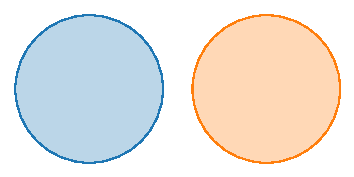
\includegraphics{figures/diagrams/connected_disks.pdf}
%     \caption[short]{The space 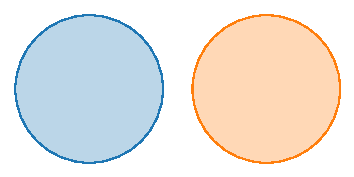
\includegraphics[height=1.5ex]{figures/diagrams/connected_disks.pdf} is disconnected as \(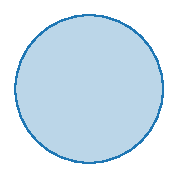
\includegraphics[height=1.5ex]{figures/diagrams/disk_blue.pdf} \^ 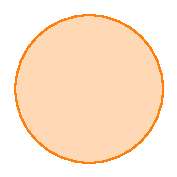
\includegraphics[height=1.5ex]{figures/diagrams/disk_orange.pdf} = \emptyset\) and \(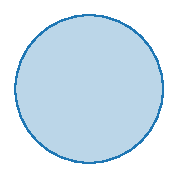
\includegraphics[height=1.5ex]{figures/diagrams/disk_blue.pdf} \u 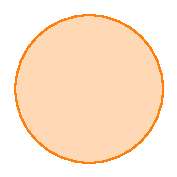
\includegraphics[height=1.5ex]{figures/diagrams/disk_orange.pdf} = 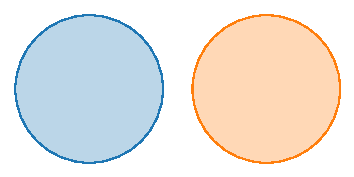
\includegraphics[height=1.5ex]{figures/diagrams/connected_disks.pdf}\)}
% \end{figure}

% A useful corollary of this is that a space is connected if and only if the only two sets in the topology that are both closed and open are \(X\) and \(\emptyset\).

% For any space that is not connected, we can turn this into a series of connected spaces by breaking it into its components. We do this by applying an equivalence relation \(p \tilde q\) if there is a connected subset of \(X\) that contains \(p\) and \(q\). The equivalence class of \(X\) under this equivalence are called the \emph{components} of \(X\), and each is connected. 

% \emphmarginnote{Path connectedness} is a stronger notion than connectedness that implies connectedness. A space is path connected if for every \(p, q \in X\), there is a continuous map \(f: \sbr{0,1} \to X\).
% \begin{figure}[h]
%     \centering
%     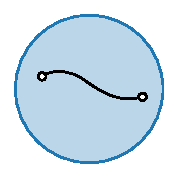
\includegraphics{figures/diagrams/continuous_path.pdf}\hspace{1cm}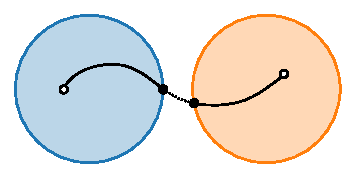
\includegraphics{figures/diagrams/discontinuous_path.pdf}
%     \caption{The space on the left is path connected, the space on the right is not.}
% \end{figure}

\section{Topological Manifolds}

\begin{definition}[Topological manifold]
	An n-dimension \emph{topological manifold} is a \emph{Hausdorff} and \emph{second-countable} topological space for which \emph{every point has a neighbourhood homeomorphic to an open subset of \(\R^n\)}.
\end{definition}
This last condition is also stated as being \emph{locally Euclidean of dimension \(n\)}.
Note that the requirement of second countability is sometimes replaced with \emphmarginnote{paracompactness}.
In locally Euclidean Hausdorff spaces, these two notions imply each other and so this is a moot point.
This means therefore a manifold \(X\) is in fact a tuple \(\del{X, \topo{X}}\), containing a set along with a suitable topology.

Euclidean space of dimension n is clearly a topological manifold of dimension n, when endowed with the topology induced by the usual Euclidean metric.

We may also be interested in manifolds that have \emph{edges}, aptly names manifolds with boundary.
\begin{definition}[Topological manifold with boundary]
	An n-dimension \emph{topological manifold with boundary} is a \emph{Hausdorff} and \emph{second-countable} topological space for which every point has a neighbourhood homeomorphic to an open subset of the n-dimension \(\mathbb{H}^n\).
\end{definition}
where \(\mathbb{H}^n\) is the \emphmarginnote{upper half-space}, \(\mathbb{H}^n = \cbrcolon{\del{x_1, ..., x_n}\in\R^n}{x_n \geq 0}\).
We call any point that has a neighbourhood homeomorphic to the upper half-space a \emphmarginnote{boundary point}, and denote the collection of these the \emphmarginnote{boundary}, denoted \(\partial X\).
Points that are not boundary points are call \emphmarginnote{interior points}.

The required structure of a manifold (with boundary) implies additional properties: all topological manifolds (with boundary) are locally path-connected, locally compact, and paracompact.

Using the previously outlined ways of producing topological spaces from other topological spaces, it is clear we can create new manifolds automatically via taking subspaces of manifolds, taking products of manifolds, or by taking direct products of manifolds.
We can also produce new manifolds via quotients, however we must check that this quotient preserves the Hausdorff and second countable properties manually.

\subsection{Bundles and Sections}

The operations just discussed can create many types of new manifold.
However, there exist a very useful class of manifold that we can study that while \emph{locally} look like the direct product of two manifolds, \emph{globally} they do not. The prototypical example of this is the M\"{o}bius strip.
\begin{figure}[h]
	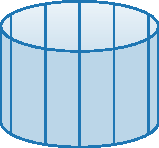
\includegraphics{figures/diagrams/cylinder.pdf}\hspace{1cm}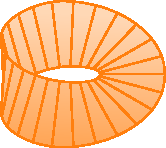
\includegraphics{figures/diagrams/mobius_strip.pdf}\caption{The Both the Möbius strip and the cylinder look a bit like the direct product of the circle and the unit interval. The cylinder is exactly this, but the M\"{o}bius strip has an additional "twist" in it.}
\end{figure}

We can make this notion more precise with the study of \emph{bundles}.
\begin{definition}[Bundle]
    A \emph{bundle} is a triple \((E, \pi, B)\) consisting of a topological space \(E\) the \emphmarginnote{total space}, \(p: E \to B\) the \emphmarginnote{projection}, a continuous surjective map, and a topological space \(B\) the \emphmarginnote{base space}.
\end{definition}
The \emphmarginnote{fibre} at a point \(p\in B\), \(F_p\), is given by the preimage of the point under the projection, \(F_p = \pi^{-1}(p)\). In the other direction, the projection map will send all points in the fibre \(F_p\) to \(p\).

Intuitively, we can think about this bundle as having "glued" all the fibres to each point on the manifold, and, in addition, we have specified thought \(E\) how fibres next to each other are to be glued together. This is glueing of the fibres to each other is how we procure the difference between the M\"{o}bius strip and the cylinder.

The simplest example of a bundle is the direct product, \((B\times F, \pi: (b, f) \mapsto b, B)\).

This is also the simplest example of a \emph{fibre bundle}, which is a restriction of the idea of a bundle, where every fibre is homeomorphic to some canonical fibre.
\begin{definition}[Fibre Bundle]
    \label{def:fibre_bundle}
    A \emph{fibre bundle} is a quadruple \((E, \pi, B, F)\) where the first three arguments are a bundle such that \[\pi^{-1}(p) = F_p \isomtop F \; \forall \; p\in B\] for an additional topological space \(F\). 
\end{definition}
The M\"{o}bius strip and the cylinder are both examples of fibre bundles.
The have the same base space, \(S^1\), and canonical fibre, \(\sbr{0,1}\), but different total space and projection.

One concept that will be very important to us is the notion of a \emph{section} of a bundle.
\begin{definition}[Section]
    A \emph{section} of a bundle \((E, \pi, B)\) is a continuous map \(\sigma: B \to E\) such that the composition of the section with the projection is the identity, i.e. that \[\pi \circ \sigma = \id_B\]
\end{definition}
Intuitively, a section defines a map that assigns to every point in \(p\in B\) a point in the fibre \(F_p\).
\todo{section picture}
In the sense of fibre bundles, we can see this as a way of defining functions from the base space into the typical fibre, but where the sense of continuity for this function can be different to that of a typical continuous function from \(B \to F\), which would correspond to the product bundle of \(B\) and \(F\).

\subsection{Charts and atlases}
While we can view manifolds as their whole, it is useful to look at them only as a patch at a time.
We can formalise this notion via charts, where we map some part of the manifold onto a subset of \(R^n\).

We call any open subset of \(X\) along with the homeomorphism \(\phi: U \to \underset{\text{open}}{\subset} \R^n\) a \emphmarginnote{chart} of \(X\).
A collection of charts \(\cbrcolon{\del{U_a, \phi_a}}{a\in A}\) such that \(\underset{a\in A}{\u} U_a = X\) an \emphmarginnote{atlas} of \(X\), denoted \(\atlas{X}\).
For any two charts \(\del{U, \phi_U}, \del{V, \phi_V}\) in an atlas where \(U\^ V \neq \emptyset\) we can define the \emphmarginnote{transition map} between them as the map \(\phi_{UV}: \phi_{U}(U\^V) \to \phi_V(U\^ V)\) as the composition \(\phi_{UV} = \phi_V \circ \phi_U^{-1}\).
An atlas is called a \emphmarginnote{maximal atlas} if it is not a subset of some larger atlas.

\begin{figure}[h]
	% 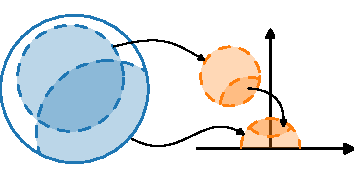
\includegraphics{figures/diagrams/boundary_charts2.pdf} % 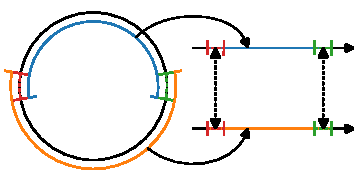
\includegraphics{figures/diagrams/circle_atlas.pdf}
	\input{figures/tex/boundary_chart.tex}
	\caption{Two charts of the atlas \(\atlas{X}\) of \(X\), the unit disk, a manifold with boundary. \(\del{U, \phi_U}\), a chart mapping into a subset of \(\R^n\), and \(\del{V, \phi_V}\), a chart mapping into a subset of the upper half-space \(\mathbb{H}^2\).}
\end{figure}
\begin{figure}[h]
	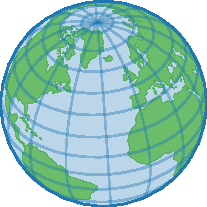
\includegraphics{figures/diagrams/earth.pdf}\hspace{1cm}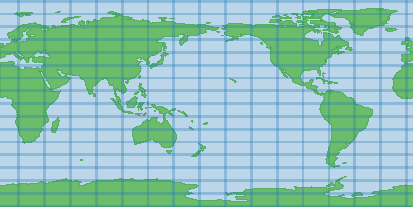
\includegraphics{figures/diagrams/earth_flat.pdf}
	\caption{The projection of the earth onto a flat map is the prototypical example of a chart.
		While the Mercator projection it looks like the chart covers the whole globe, but mathematically it is in fact missing the poles and a line connecting them as we need the set to be an open one.
	}
\end{figure}

While not required for the definition of a manifold, the concept of charts and atlases is key to the study of additional structure we can impose on a manifold.
In addition, from a computational perspective they are incredibly useful as they give us one way of representing points on a manifold as a series of real numbers.



\todo[inline]{Some examples of manifolds, and the various production operations.}

\section{Differentiable and Smooth Manifolds}

To add additional structure to our manifolds, we might require that the atlas we specify has some additional properties.
For any property, \ding{110}, we say that an atlas is \ding{110}-compatible if for all pairs of charts in the atlas the transition map between charts has the particular property. We call a manifold equipped with an atlas that is \ding{110}-compatible a \ding{100}-manifold.

By definition, all atlases are \(C^0\), and so all manifolds are \(C^0\)-manifolds.
In addition, we could require our manifold to be a \emphmarginnote{(\(C^k\))-differentiable manifolds}, where all the transition maps are \(C^k\), i.e. they have up to \(k\) differentials.
Of most interest to us will be \emphmarginnote{smooth manifolds}, manifolds for which the transition maps are infinity differentiable, i.e. they are in \(C^\infty\).

A \emphmarginnote{smooth structure} on \(X\) is a \emph{maximal smooth atlas}, and so a \emphmarginnote{smooth manifold (with boundary)} is a triple \((X, \topo{X}, \atlas{X})\) with the right properties.
Every coordinate chart of a smooth manifold is itself smooth.

Showing a manifold is smooth is not always simple from the definition.
The following is useful as it lets us create a smooth manifold with suitable charts: \begin{lemma}[Smooth manifold chart lemma] \label{lem:smooth_chart} Suppose \(X\) is a set, and we have a subset of collections \(\cbr{U}_a\) along with maps \(\phi_a: U\to \R^n\).
	If the following are satisfied: \1 for each \(a\), \(\phi_a\) is a bijection between \(U_a\) and an \emph{open} subset of \(\R^n\) with the usual topology.
	\2 For each \(a\), \(b\), the sets \(\phi_a(U_a\^U_b)\) and \(\phi_b(U_a\^U_b)\) are open in \(\R^n\) with the usual topology.
	\3 For all \(a,b\) where \(U_a\^U_b \neq \emptyset\), the map \(\phi^{-1}_a\circ\phi_b: \phi_a(U_a\^U_b) \to \phi_b(U_a\^U_b)\) is smooth.
	\4 Countably many \(U_a\) cover \(X\).
	\5 When \(p, q\in X\), \(p\neq q\), there exists some \(U_a\) containing \(p\) and \(q\), or there exist disjoint \(U_a, U_b\) with \(p\in U_a\), \(q\in U_n\).
	\0
	Then \(X\) has a unique smooth manifold structure such that each \((U_a, \phi_a)\) is a smooth chart.
\end{lemma}
\begin{proof}
	\cite[p.22]{lee2013smooth}
\end{proof}
The topology of the structure is induced by the topology on \(\R^n\) and the \((U_a, \phi_a)\) (1-3).
The basis for the topology on \(X\) is given by \(\basis = \cbrcolon{\phi_a^{-1}(S)}{S \text{ is open in } \phi_a(U_a) \text{ for all } a}\).
4. ensures second countability, and 5.
Hausdorff.

We can define \emphmarginnote{smooth functions on manifolds}.
\(f: X\to \R^k\) is a smooth function if for every point \(p \in X\) and chart \((U, \phi) \in \atlas{X}\) the function \(f \circ \phi^{-1}: \phi(U)\to \R^k\) is smooth.
Typically, we denote the space of smooth function \(f: X\to \R^k\) as \(C^\infty(X, \R^k)\), and \(f: X\to \R\) \(C^\infty(X)\).
Like continuity, smoothness is a local property, and it suffices to check that for a sub-atlas of the atlas on a smooth manifold that a function is smooth on the restriction ot each chart to show it is globally smooth.

We can define \emphmarginnote{smooth functions between manifolds} as well.
\(f: X \to Y\), where \(X, Y\) are smooth manifolds, is smooth if for each pair of charts \((\phi, U)\in \atlas{X}, (\psi, V) \in \atlas{Y}\) the composition \(\psi \circ f \circ \phi^{-1}: \phi(U)\to \psi(V)\) is smooth.
We denote the space of smooth functions between \(X\) and \(Y\) as \(\C^\infty(X, Y)\).
A \emphmarginnote{diffeomorphism} between manifolds is a smooth bijection with smooth manifolds.
A pair of manifolds for which a diffeomorphism exists are said to be \emphmarginnote{diffeomorphic}, \(X \isomdiff Y\).

\begin{figure}[h]
	\documentclass[tikz,10pt]{standalone}
\usepackage[standalone,commands]{../../MJH}

\graphicspath{/Users/mhutchin/Documents/thesis/figures/diagrams/}

% \usepackage{tikz}
% \usetikzlibrary{positioning}

\usepackage{pgfplots}
\pgfplotsset{compat=1.17}
% \usepgfplotslibrary{external}
% \usepgfplotslibrary{groupplots}
% \usepgfplotslibrary{fillbetween}
% \usetikzlibrary{fadings}

\begin{document}
    % \tikzsetnextfilename{generative_model}
    \begin{tikzpicture}
        \node (simple) at (0,0) {
\includegraphics{/Users/mhutchin/Documents/thesis/figures/diagrams/hom_not_diff.pdf}};
        \node (math) at (0, 0.5) {\(\isomtop\)};
        \node (math) at (0, -0.5) {\(\not\isomdiff\)};
    \end{tikzpicture}
\end{document}
	\caption{Diffeomorphism is a stronger condition that homeomorphic.
		The disk is homeomorphic to the square, but not diffeomorphic, as one runs into smoothness difficulties with the sharp corners.
	}
\end{figure}

\section{Tensors}
Having introduced differentiable structure to manifolds, we are ready to start talking about derivatives on manifolds.
Derivatives naturally form a vector space in multivariate calculus.
Therefore, we briefly recap vector spaces, and discuss the notion of tensors.
Tensors will be central to the study of deep structure on manifolds later.

\subsection{Algebraic structures}

Briefly, we recall the definitions of a few algebraic structures.

\begin{definition}[Group]
	A \emph{group} is a set \(G\) and an operation \(\cdot: G\times G\to G\) such that 
	\begin{enumerate}
		\item For \(a,b\in G\), \(a \cdot b \in G\).
		\item The operation is \emph{associative}, for \(a, b, c \in G\), \((a \cdot b) \cdot c = a \cdot (b\cdot c)\).
		\item There exists an \emph{identity element} \(e\in G\) such that for any \(a \in G\), \(e\cdot a = a \cdot e = a\).
		\item For every element \(a \in G\), there is another element \(a^{-1} \in G\) such that \(a \cdot a^{-1} = e = a^{-1}\cdot a\), its \emph{inverse}.
	\end{enumerate}
\end{definition}

\begin{definition}[Abelian group]
	An \emph{Abelian group} is a group \((G, \cdot)\) where in addition \(\cdot\) is \emph{commutative}, i.e. for \(a, b \in G\), \(a \cdot b = b \cdot a\).
\end{definition}

\begin{definition}[Field]
	A \emph{field} is a set \(F\) equipped with two maps, \(+: F\times F\to F\) and \(*: F\times F\to F\) such that
	\begin{itemize}
		\item \((F, +)\) is an Abelian group, with identity element \(0\).
		\item \((F\backslash\cbr{0}, *)\) is an Abelian group with identity element \(1\).
	\end{itemize}
	In addition the operations \emph{distribute} in the following way, for \(a, b, c \in F\),
	\[(a + b) * c = a*c + b*c\]
\end{definition}

The prototypical example of a field is the real numbers, \(R\), equipped with the usual addition and division, excluding division by zero. The complex, \(\C\), and rational, \(Q\) numbers are also fields.

Also of use the weaker definition of a \emph{ring}.

\begin{definition}[Ring]
	\label{def:ring}
	A \emph{ring} is a set \(F\) equipped with two maps, \(+: F\times F\to F\) and \(*: F\times F\to F\) such that
	\begin{itemize}
		\item \((F, +)\) is an Abelian group, with identity element \(0\).
		\item For \((F\takeaway\cbr{0}, *)\), the \(*\) operator only satisfies associativity, for \(a, b, c \in F\takeaway\cbr{0}\), \((a \cdot b) \cdot c = a \cdot (b\cdot c)\)
	\end{itemize}
\end{definition}

This definition is useful for when discussing spaces of functions, for example the square integrable functions on some domain \(D\), \(L^2(D)\).
In this case, if we define the addition operation in the usual pointwise way, the identity function (the constant zero function) is not the only function we need to exclude to make division by a function sensible.
We would need to exclude any function with a zero at any point.
For this same reason, defining the inverse of a function under multiplication is not sensible, as the inverse of the points in a function that are zero are undefined.
If we were to restrict ourselves to strictly positive \(L^2\) functions, then we could form a field from these.
As it stands however this is not so useful, so we satisfy ourselves with a ring.


\subsection{Vector Spaces}
\begin{definition}[Vector space over a field]
	A \emph{vector space} over a field \(F\) is a set \(V\) equipped with a \emph{vector addition} operation \(\oplus: V\times V \to V\) and a \emph{scalar multiplication} operation \(\odot: F \times V \to V\) such that 
	\begin{itemize}
		\item \((V, \oplus)\) is an Abelian group.
		\item \(\odot\) is an \emph{action} on \((V, \oplus)\) such that
		\begin{enumerate}
			\item Scalar multiplication distributes over vector addition, for \(\lambda \in K\), \(v, w \in V\), \(\lambda \odot (v \oplus w) =  (\lambda \odot v) \oplus (\lambda \odot w)\).
			\item Field addition distributes over vector addition, for \(\lambda, \mu \in K\), \(v \in V\), \((\lambda + \mu)\odot v =  (\lambda \odot v) \oplus (\mu \odot v)\).
			\item Field multiplication is compatible with scalar multiplication, for \(\lambda, \mu \in K\), \(v \in V\), \((\lambda * \mu)\odot v =  \lambda \odot (\mu \odot v)\).
			\item The field identity is preserved, for \(v\in V\), \(1 \odot v = v\).
		\end{enumerate} 
	\end{itemize}
\end{definition}
When discussing different vector spaces over the same field, properly one should denote their vector addition and scalar multiplication operations with different notation, e.g. \(\oplus, \boxplus\), to differentiate these operations from each other and the field operations.
Typically, however this is suppressed and the same symbol is used for field multiplication and addition, as well as the vector counterparts on different vector spaces as one can infer the correct operation from context.
We will use this convention.

A \emphmarginnote{topological vector space} is a vector space over a topological field, equipped with a topology so that vector addition and scalar multiplication are continuous.
Most commonly we deal with vector spaces over the \emph{real numbers} \(\R\), but sometimes also over the \emph{complex numbers} \(\C\).
From now on we will only discuss real vector spaces.

A subset of a vector space that is closed under the vector operation is called a \emphmarginnote{linear subspace}, distinct from a topological subspace.
If we have a finite set of vectors \(S = \cbr{v_1, .
	.., v_n}, v_i \in V\), a \emphmarginnote{linear combination} of them is denoted by \(\sum_{i=1}^n a_i v_i\) with \(a_i \in \R\).
The \emphmarginnote{span} of a set of vectors, denoted \(\Span(S)\) is the set of all linear combinations of the vectors, and is a linear subspace.
If \(V = \Span(S)\) then \(S\) \emph{spans} \(V\).
A set \(S\) is said to be \emphmarginnote{linearly dependent} is there exist \(a_i\in \R\) such that the linear combination is \(0\in V\).
Otherwise, they are \emphmarginnote{linearly independent}.

\textcolor{red}{some inf dim one?}

A \emphmarginnote{linear map} between vector spaces \(V\) and \(W\) are maps \(T: V \to W\) such that they preserve the structure of vector addition and scalar multiplication.
I.e. \(T(av + bw) = aT(v) + bT(w)\).
A map \(T: V \to \R\) is called a \emphmarginnote{linear functional}.
The \emphmarginnote{image} of \(T\), \(\im T\) is the set \(\im T = \cbrcolon{w = T(v)}{v \in V}\).
The \emphmarginnote{kernel} or \emphmarginnote{null space} of \(T\), \(\ker T\) is the preimage of \(0\) under \(T\), \(\ker T = \cbrcolon{v}{T(v) = 0, v\in V}\).

If \(V, W\) are vector spaces over the same field, a bijective linear map \(T: V \to W\) then \(T\) is called a \emphmarginnote{vector isomorphism}, \(T\) has an inverse, and \(V, W\) are said to be (vector) isomorphic, \(V \isomvec W\).

The space of all linear maps from a vector space \(V\) to a vector space \(W\) over the same field is denoted as \(\Hom(V, W)\), the \emphmarginnote{homeomorphisms} from \(V\) to \(W\).
This space of homeomorphisms can in fact be itself turned into a vector space by defining vector addition
\[
	\boxplus: 	\Hom(V, W) \times \Hom(V, W) &\to \Hom(V, W) \\
	(f \boxplus g)(v) &\mapsto f(v) + g(v) 
\]
and scalar mutliplication
\[
	\boxdot: K \times \Hom(V, W) &\to \Hom(V, W) \\	
	(\lambda \boxdot f)(v) = \lambda f(v)
\]
An \emphmarginnote{endomorphism} of \(V\) is a linear map onto itself, and the space of these \(\End(V) = \Hom(V,V)\).
An \emphmarginnote{automorphism} of \(V\) is a linear isomorphism onto itself, and the space of these is \(\Aut({X}) = \cbrcolon{f\in \End{V}}{f \text{ is an isomorphism}}\).

For any vector space \(V\), we can define a \emphmarginnote{covector} as a linear map \(\omega: V \to \R\).
We call the space of covectors the \emphmarginnote{dual space} of \(V\), denoted \(V^*\), and it is equal to \(\Hom(V, K)\), where \(V\) is a vector space over the field \(K\).

For any linear map \(A: V\to W\), we can define its \emphmarginnote{dual map}, \emph{transpose}, or \emphmarginnote{adjoint} \(A^*: W^* \to V^*\) as the map \[(A^*\omega)(v) = \omega(Av), \quad \omega \in W^*, v \in v\].
This adjoint distributes over composition, but reverse terms, \((A\circ B)^* = B^* \circ A^*\), and preserves the identity, \((\id_V)^* = \id_{V^*}\).

The \emphmarginnote{double dual} of \(V\), \(V^{**} = (V^*)^*\), the dual of the dual, for finite dimension vector spaces is isomorphic to the original space \(V\).
There is a natural map \(\xi: V \to V^{**}\) as \[\xi(v)(\omega) = \omega(v) \quad, \omega \in V^*, v \in V\].
Because we can unambiguously identify \(V\) with \(V^{**}\) for finite dimension vector spaces, we typically only talk about \(V\) and its dual \(V^*\).
Sometimes one may see the inner product between a vector and a covector written as \(\innerprod{\omega}{v}\) or \(\innerprod{v}{\omega}\).
The second denotes the action of \(\xi(v)\) on \(\omega\), but the result of both are identical.

\subsection{Tensors}
\label{sec:tensors}

% \subsection{Higher order tensors}
% \label{sec:higher_order_tensors}
Covectors defined linear maps over vector spaces.
Tensors allow us to define \emphmarginnote{multilinear maps}.
For vector spaces \(V_1, .
.., V_k, W\), a multilinear map is a map \(f: V_1 \x ... \x V_k \to W\) if for any \(i\), \[f(v_1, ..., a v_i + b v'_i, ..., v_k) = a f(v_1, ..., v_i, ..., v_k) + b f(v_1, ..., v'_i, ..., v_k)\].
Tensors are multilinear maps over copies of the same vectors space and its dual.
We can define the following spaces of multilinear maps 

\begin{tabular}{lcc} \scshape Map                                                                                                  & \scshape Notation           & \scshape "Archaic" name             \\ \(f: \underbracket{V\x .
               .. \x V}_{k \text{ copies}} \to \R \)                                                                               & \(T^k(V^*) = T^{(0,k)}(V)\) & covariant \(k\)-tensor on \(V\)     \\
               \(f: \underbracket{V^* \x ... \x V^*}_{k \text{ copies}} \to \R \)                                                  & \(T^k(V) = T^{(k,0)}(V)\)   & contravariant \(k\)-tensor on \(V\) \\
               \(f: \underbracket{V^*\x ... \x V^*}_{k \text{ copies}}\x \underbracket{V \x ... \x V}_{l \text{ copies}} \to \R \) & \(T^{(k,l)}(V)\)            & mixed \((k,l)\)-tensor on \(V\)     \\
\end{tabular}

The "archaic" name refers to how the basis coefficients transform with the basis vectors.
\emph{Covariant} tensor basis coefficients transform \emph{with} them, and \emph{contravariant} \emph{opposite} to them.
In the modern setting where we typically work basis-free these make less sense.
By convention, and for sensible reasons, the a tensor in \(T^{(0,0)}\) is just a scalar.

The \emphmarginnote{tensor product} is an operation \(\otimes: T^{(k,l)}(V) \x T^{(p,q)}(V)\to T^{(k+p, l+q)}(V)\).
It is defined by its evaluation \[\del{F\otimes G}(\omega^1, .
	.., \omega^k, \omega^{k+1}, ..., \omega^{k+p}, v_1, ..., v_l, v_{l+1}, ..., v_{l+q})\\ = F(\omega^1, ..., \omega^k, v_1, ..., v_l) G(\omega^{k+1}, ..., \omega^{k+p}, v_{l+1}, ..., v_{l+q})\].
This is an associative but \emph{not} a commutative operation.

Some immediately interesting tensor spaces arise
\begin{itemize}
	\item \(T_1^0V = \Hom(V) = V^*\)
	\item \(T_1^1V = V \otimes V^*\). This is in fact isomorphic to \(\End(V^*)\).
	To see this, note that for a fixed \(\omega \in V^*\), and \(T\in T_1^1V\), \(T(\cdot, \omega): V\to F\), and since this is a linear map, this must be an element of \(V^*\). 
\end{itemize}

\todo{write about the trace - find a concise way to state the coordinate free theory}

\todo{write about tensors corresponding to linear operators}

\subsection{Bases}
\label{sec:vector_bases}
The concepts introduced so far are abstract, and have no easy way to be represented in a computer or on paper and manipulated numerically.
In order to do this, we will need to express vectors in a \emph{basis}.

A \emphmarginnote{Hamel basis} for \(V\) is a linearly independent subset \(S \subseteq V\) such that \(\Span(S) = V\).
Every \(v\in V\) has a \emph{unique} expression as a linear combination of the basis.
The choice of basis is non-unique, although often there is a sensible choice.
All bases of a vector space are of the same cardinality, called the dimension of the space, \(\dim V\).
If the basis is finite of size \(n\), the space is said to be finite-dimension or \(n-\)dimension.
If it is infinite, infinite-dimension.
If we can ascribe an order to a basis (if it is finite or countable) then we call it an \emphmarginnote{ordered basis}, and we can identify the elements \(v\in V\) of the vector space with the ordered set of field coefficients \(\del{a_i1, .
	..}\) such that \(\sum_i a^i v_i  = v\).
This is called the \emphmarginnote{basis representation}.
All bases of the same vector space are of the same dimension.

For a finite dimension vector space then it is common to express a vector as an ordered list of numbers, with each element of the list being a basis coefficient of the vector expressed in a basis,
\[v = \sum_{i=1}^n v^ie_i = \begin{bmatrix}
	v_1 \\ \vdots \\ v_n
\end{bmatrix}\]

For a finite dimension vector space, if we have a basis on \(V\), \(e_1, .
.., e_n\), then we can define the \emphmarginnote{standard dual basis} \(\epsilon^1, ..., \epsilon^n\) on \(V^*\) by \(\epsilon^i(e_j) = \delta^i_j\), showing it is also \(n\)-dimension.
Note the use of upper indices, inline with Einstein summation notation.
We write basis vectors of the dual space with upper indices so that they appear once upper and once lower when computing the interaction of a vector and a covector.
\[\omega(v) = (\omega_i\epsilon^i)(v^je_j) = \omega_iv^j \epsilon^i(e_j) = \omega_iv^j \delta^j_i = \omega_i v^i\]

We can build a \emphmarginnote{basis on a tensor space} then out of the basis on \(V\) and \(V^*\), giving basis elements of the form \[e_{i_1}\otimes .
	..\otimes e_{i_k}\otimes \epsilon^{j_1},  \otimes ...\otimes \epsilon^{j_l}, \quad\quad i_{a}\in [1,..., k], \; j_b \in [1,..., l]\] with the obvious action on basis vectors \[e_{i_1}\otimes ...\otimes e_{i_k}\otimes \epsilon^{j_1},  \otimes ...\otimes \epsilon^{j_l}\del{\epsilon^{s_1}, ..., \epsilon^{s_k}, e_{t_1}, ..., e_{t_l}} = \delta^{s_1}_{i_1} ... \delta^{s_k}_{i_k} \delta^{j_1}_{t_1} ... \delta^{j_l}_{t_l} \].
This makes a \(T^{(k,l)}V\) an \(n^{k+l}\)-dimension vector space.
For a tensor \(T\in T_q^pV\), we can express this in basis coefficients 
\[T = \underbrace{\sum_{a_1=1}^n ... \sum_{b_q =1}^n}_{p+q\text{ sums}} T_{b_1, ..., b_q}^{a_1, ...a_p} e_{a_1}\otimes...\otimes e_{a_p} \otimes \epsilon^{b_1}\otimes...\otimes \epsilon^{b_q}\]

For a linear map \(f\) between finite dimension vectors spaces, \(V, W\), each with a basis \(e_1^V, ..., e_n^V\), \(e_1^W, ..., e_m^W\), the \emph{components} of the map can be expressed by the coefficients \(f^i_j = f(e_i^V, e_j^W)\).
For a vector \(v\in V\) expressed in the basis, \(v = \sum_{i=1}^{n} v^i e_i^V\), its image under the linear map \(f\), \(f(v)\), can then be expressed in coordinates in the basis on \(W\) as \(w = f(v) = \sum_{j=1}^{m} (\sum_{i=1}^n f_i^j v^i) e_j^W = \sum_{j=1}^m w^j e_j^W\).

A \emph{change of basis} of a vector can be performed between two different bases \(e_1, ..., e_n\) and \(\tilde e_1, ..., \tilde e_n\).
Each basis vector \(\tilde e_j\) can be expressed as a linear combination of the first basis, \(\tilde e_j = \lambda_j^i e_i\).
Any vector expressed in the first basis, \(v = v^i e_i\) can then be re-expressed in the second basis via \(v = \tilde v^j \tilde e_j\) where \( \tilde v_j = \lambda^j_i v^i\).
Similarly we can 
As such we can see a change of basis as an automorphism of \(V\).

% \(n\)\emph{-dimension Euclidean space}\marginnote{\(n\)-dimension Euclidean space}, \(\R^n\) is the prototypical example of a finite-dimension real vector space with vector and scalar multiplication defined by\[(x_1, ..., x_n) + (y_1, ..., y_n) &= (x_1 + y_1, ..., x_n + y_n) \\ a(x_1, ..., x_n) &= (ax_1, ..., ax_n)\], with standard basis \((e_1, ..., e_n)\), \(e_i = (0,..., 1, ..., 0)\) with the \(1\) in the i'th position.

\subsection{Einstein summation convention}
\todo{...}

\subsection{Symmetric tensors}
\label{sec:sym_alt}
For the space of tensors of one type only (\(T^k(V^*) = T^{(0,k)}(V)\) or \(T^k(V) = T^{(k, 0)}(V)\)) we can define two special types of tensor.
We will focus here on \(T^k(V^*)\) tensors, but the same applies identically to \(T^k(V)\) tensors.

A \emphmarginnote{symmetric tensor} is one such that if you take any set of vectors \(v_1, .
.., v_k\) and permute a pair, then the evaluation of the tensor remains the same.
I.e. \[F(v_1, v_i, .
	.., v_j ...., v_k) = F(v_1,v_j, ..., v_i, ..., v_k)\].
This implies \emph{any} permutation of arguments by \(\sigma \in S_k\), the group of permutation of \(k\) elements, leave it unchanged.
We denote this \emph{linear} subspace of \(T^k(V^*)\) as \(\Sigma^k(V^*)\).
The tensor product does \emph{not} preserve symmetry.
We can \emphmarginnote{symmetrise a tensor}, denoted \(\sym F\) by \[(\sym F) (v_1, .
	.., v_k)  = \frac{1}{k!}\sum_{\sigma \in S^k}
	F\del{v_{\sigma(1)}, .
		.., v_{\sigma(k)}}\].
We can then define the \emphmarginnote{symmetric product} of \(F\in \Sigma^k(V^*), G\in \Sigma^l(V^*)\) as \[ FG = \sym (F\otimes G) \], \(FG \in T^{k+l}(V^*)\).
This is a \emph{bilinear, associative, commutative} operation.
On 2 1-tensors this gives \[\omega\eta = \frac{1}{2}\del{\omega\otimes \eta + \eta\otimes \omega}\].
All 0- and 1-tensors are symmetric trivially.

\subsection{Alternating tensors}
An \emphmarginnote{alternating tensor} is one such that if you take any set of vectors \(v_1, .
.., v_k\) and permute a pair, then the evaluation of the tensor flips sign.
I.e. \[F(v_1, v_i, .
	.., v_j ...., v_k) = -F(v_1,v_j, ..., v_i, ..., v_k)\].
This implies that \emph{even} permutations of \(S_k\) (made up of an even number of pair flips) leaves the sign unchanged and that \emph{odd} permutations flip i, \[F(v_{\sigma(1)}, .
	.., v_{\sigma(k)}) = \sign(\sigma) F(v_1, ..., v_k)\].
We denote this \emph{linear} subspace of \(T^k(V^*)\) as \(\Lambda^k(V^*)\).
The tensor product does \emph{not} preserve alternation.
We can define the \emphmarginnote{alternation of a tensor}, denoted \(\alt F\) by \[(\alt F) (v_1, .
	.., v_k)  =\frac{1}{k!}\sum_{\sigma \in S^k} \sign(\sigma) F\del{v_{\sigma(1)}, ..., v_{\sigma(k)}}\].
For any tensor, this returns us an alternating tensor.

Let \(I = \del{i_1, ..., i_k}\) define a \emphmarginnote{mutli-index}.
Let \(I_\sigma = \del{i_{\sigma(1)}, ..., i_{\sigma(n)}}\).
Assume we have a basis for \(V^*\), \(\epsilon^1, ..., \epsilon^n\).
We can define an \emphmarginnote{elementary alternating tensor} by its action on \(k\) vectors, \(v_1, ..., v_k\) 
\[\epsilon^I (v_1, ..., v_k) = \det \begin{bmatrix}
	\epsilon^{i_1}(v_1) & \dots & \epsilon^{i_1}(v_1)\\
	\vdots & \ddots & \vdots \\
	\epsilon^{i_k}(v_1) & \dots & \epsilon^{i_k}(v_k)
\end{bmatrix} 
\] where \(\det\) is the usual determinant. 
If we express the vectors \(v_1, ..., v_k\) in the dual basis to \(\epsilon^1, ..., \epsilon^n\), \(e_1, ..., e_n\), then this is 
\[\epsilon^I (v_1, ..., v_k) = \det \begin{bmatrix}
	v_1^{i^1} & \dots & v_k^{i^1}\\
	\vdots & \ddots & \vdots \\
	v_1^{i^k} & \dots & v_k^{i^k}
\end{bmatrix} 
\].
Clearly this is an alternating tensor, as swapping any two columns in the determinant results in the change in a sign, and it is zero if any two vectors are colinear.

Evaluating an elementary alternating tensor on basis elements \(e_{j_1}, ... e_{j_k}\) gives 
\[\epsilon^I(e_1, ..., e_k) = \begin{bmatrix}
	\delta_{j_1}^{i^1} & \dots &\delta_{j_k}^{i^1}\\
	\vdots & \ddots & \vdots \\
	\delta_{j_1}^{i^k} & \dots & \delta_{j_k}^{i^k}
\end{bmatrix} = \delta_J^I\], where \(J=(j_1, ..., j_k)\).

By picking a subset of the elementary alternating tensors we can produce a basis on the space of alternating tensors.
We need to exclude any that are zero (\(I\) with repeated indicies) and any \(I\) that is a permutation of another element of the basis set. 
For the space alternating tensors \(\Lambda^k(V^*)\) over an \(n\)-dimension vector space \(V^*\), we can therefore pick the basis
\[  \cbrcolon{\epsilon^I}{ I \text{ is a strictly increasing multiindex of size } k} \].


The \emphmarginnote{wedge product} of two alternating tensors, enoted by \(\wedge\), maps two alternating tensors to an alternating tensor of higher dimension, \[\wedge: \Lambda^k(V^*) \times \Lambda^l(V^*) \to \Lambda^{k+l}(V^*) \].
For \(F\in \Lambda^k(V^*), G\in \Lambda^l(V^*)\), is is defined as \[ F\wedge G = \frac{(k+l)!
	}{k!l!} \alt (F\otimes G) \], \(F\wedge G \in  \Lambda^{k+l}(V^*)\).
This is a \emph{bilinear, associative, anti-commutative} (\(F\wedge G = \del{-1}^{kl}G\wedge F\)) operation.
All 0- and 1-tensors are alternating trivially.

The \emphmarginnote{interior product} is an operation \(\iprod: \Lambda^k(V^*) \x V \to \Lambda^{k-1}(V^*)\) defined by \[(v\iprod \omega)(w_1, .
	.., w_{k-1}) = \omega(v, w_1, ..., w_{k-1})\].

Finally, we define the notion of a \emphmarginnote{volume form}.
For an \(n\)-dimension vector space \(V\), a volume form is a tensor \(\omega\in \Lambda^n V\).
For a series of vectors \(v_1, ..., v_n\), the \emph{volume} they span is given by
\[
	\vol(v_1, ..., v_n)	= \omega(v_1, ..., v_n)	
\]
If the set of vectors are not linearly independent, this volume spanned will be zero.
Intuitively this makes sense as then the vectors span a hyperplane in \(V\), which should have zero volume in the whole of \(V\). 

\section{Tangent, cotangent, and tensor spaces}
\subsection{Tangent spaces and derivations}
\label{sec:tangents_derivations}

One of the key advantages of studying smooth manifolds is that it allows us to bring the notions of calculus to the study of manifolds.
The most basic concept is that of the \emph{tangent vector}.

We can begin looking at tangent vectors on manifolds by first looking at tangent vectors on \(\R^n\).
Since all we have defined on smooth manifolds so far is smooth functions and smooth charts, we will need a definition that works in terms of these.
Consider the set \(\R^n_p = \cbr{p}\x \R^n\).
We will call this the \emphmarginnote{geometric tangent space} at \(p\).
We call an element of this, \((p, v), \; v\in \R^n\), usually written at \(\eval{v}_p\) or \(v_p\), a \emphmarginnote{geometric tangent vector}.
This is clearly a vector space with operations \[v_p + w_p = (v + w)_a \quad\quad c(v_p) = (cv)_p\].
The subscript \(p\) is to allow us to differentiate between tangent spaces at different points \(p\) and \(q\).
Given the canonical basis of \(\R^n\), \(e_1, .
..., e_n = (1, ..., 0), ..., (0, ..., 1)\), we can put a natural basis on \(\R^n_p\) as \(\eval{e_1}_p = (p, e_1), ..., \eval{e_n}_p = (p, e_n)\) via the \emphmarginnote{canonical isomorphism} \(\inclusion_p: \R^n \to \cbr{p}\x \R^n\), \(\inclusion_p : v \mapsto (p, v)\).

For a smooth function \(f \in C^\infty(\R^n)\) we can define the \emphmarginnote{directional derivative} \(D_{v_a}: C^\infty(\R^n) \to \R\) as \[ D_{v_a} f = D_v f(a) = \eval{\od{}{t}}_{t=0} f(a + tv) \].
This operation obeys the product rule \[ D_{v_a} (fg) = f(a) D_{v_a}f + g(a) D_{v_a}f \].
For the basis vectors \(\eval{e_i}_p\), \[D_{\eval{e_i}_p} f = \pd{f}{x_i}(p)\], simply the partial derivative with respect to the \(i\)th input.
So for \(v_p \in \R^n_p\) expressed as \(v = \sum_{i=1}^n v_i \eval{e_i}_p\), we have that \[D_{v_p} f = \sum_{i=1}^n v_i \pd{f}{x_i}(p)\] \begin{figure}[h] \documentclass[tikz,10pt]{standalone}
\usepackage[standalone,commands]{../../MJH}

\graphicspath{/Users/mhutchin/Documents/thesis/figures/diagrams/}

% \usepackage{tikz}
% \usetikzlibrary{positioning}

\usepackage{pgfplots}
\pgfplotsset{compat=1.17}
% \usepgfplotslibrary{external}
% \usepgfplotslibrary{groupplots}
% \usepgfplotslibrary{fillbetween}
% \usetikzlibrary{fadings}

\begin{document}
    % \tikzsetnextfilename{directional_derivative}
    \begin{tikzpicture}
        \node (simple) at (0,0) {
\includegraphics{/Users/mhutchin/Documents/thesis/figures/diagrams/directional_derivative.pdf}};
    \end{tikzpicture}
\end{document} \caption{Directional derivative.
	}
\end{figure}

\subsubsection{Tangent vectors as algebraic structures}
With this intuitive definition in mind, let us take another look at the space of smooth functions, \(C^\infty(\R^n)\).
We recall a few more algebraic definitions.
\begin{definition}[Algebra over a field]
	An \emph{algebra} \(A\) over a \emph{field} \(F\) is a set \(A\) with 3 operations,
	\begin{itemize}
		\item[] \(+:A\times A\to A\)
		\item[] \(\cdot: F \times A \to A\)
		\item[] \(\bullet: A\times A\to A\)
	\end{itemize} where
	\begin{itemize}
		\item \((A, +, \cdot)\) forms a \emph{vector space} over \(F\) 
		\item and \(\bullet\) is \emph{bi-linear} product with respect to the field \(F\).
	\end{itemize}
\end{definition}
Additionally this can be \emph{associative} if the product is associate, \emph{unital} if the product has an identity element, and \emph{commutative} if the product commutes.

We can make the space of smooth functions \(C^\infty(\R^n)\) an associative, unital, commutative algebra over the field \(\R\) by setting 
\begin{itemize}
	\item[] \(+: C^\infty(\R^n)\times C^\infty(\R^n) \to C^\infty(\R^n)\) to be pointwise addition of functions.
	\item[] \(\cdot: \R \times C^\infty(\R^n) \to C^\infty(\R^n) \) to be pointwise multiplication by a scalar.
	\item[] \(\bullet:C^\infty(\R^n)\times C^\infty(\R^n) \to C^\infty(\R^n) \) to be pointwise multiplication of functions.
\end{itemize}.
Often for this particular algebra, we will suppress the notation of \(f \bullet g\) to simply \(fg\) for \(f, g \in C^\infty(\R^n)\).

\begin{definition}[Derivation on an algebra]
	For an algebra \(A\), a \emph{derivation} is a linear map \(D: A\to A\) satisfying the product rule over the algebra product, for \(f, g \in A\),
	\[D(f \bullet g) = D(f)\bullet g + f \bullet D(g)\]	
\end{definition}
We denote the space of derivations as \(\Der A\).

For our algebra of smooth functions \(C^\infty(\R^n)\), we can restrict these derivations to a point \(p\in \R^n\)
\begin{definition}[Derivation on \(\C^\infty(\R^n)\) at \(p\in \R^n\)]
	For the algebra \(C^\infty(\R^n)\) and a point \(p\in\R^n\), a \emph{derivation at p} is a linear map \(D: C^\infty(\R^n)\to C^\infty(\R^n)\) satisfying a reduced product rule over the algebra product, for \(f, g \in C^\infty(\R^n)\),
	\[D(f \bullet g) = D(f)\bullet g(p) + f(p) \bullet D(g)\]	
\end{definition}
We denote the space of derivations as \(\Der_p C^\infty(\R^n)\).
This space of derivations at a point form a \emph{vector space} over the \emph{field} \(\R\) by defining vector addition of derivations by 
\[[(D + \tilde D)f](p) = [Df](p) + [\tilde Df](p), \quad D, \tilde D\in\Der_p C^\infty(\R^n), \; f \in C^\infty(\R^n),\; p\in \R^n \]
and scalar multiplication as 
\[[(\lambda D)f](p) = \lambda [D f](p), \quad D\in\Der_p C^\infty(\R^n), \; f \in C^\infty(\R^n),\; p\in \R^n, \; \lambda \in \R \].

We can then prove that our directional derivative and the derivations at \(p\) are isomorphic.
\begin{proposition}[\(\Der_p C^\infty(\R^n) \isomvec \R^n_p\)]
	\1 For each \(v_p\in \R^n_p\), \(D_{v_p}\) is a derivation.
	\2 The map \(v_p \mapsto D_{v_p}\) is an isomorphism from \(\R^n_p\) onto \(\Der_p C^\infty(\R^n)\).
	\0
\end{proposition}
\begin{proof}
	\cite[proposition 3.2]{lee2013smooth}
\end{proof}
This therefore connects the intuitive idea of directional derivatives that we are used to when working with Euclidean space with the more abstract definition of the vector space of derivations on the algebra of smooth functions at a point.
We call the space of derivations at a point the \emphmarginnote{tangent space}, and denote it \(T_p\R^n = \Der_p C^\infty(\R^n)\).

This then give us a natural way to define the \emphmarginnote{tangent space at a point on a manifold}.
For a manifold and a open set of the manifold \(U\subset X\), we say that a \emphmarginnote{deivation on \(C^\infty(U)\) at \(p\in U\)} is a linear map \(D:C^\infty(U) \to R\) satisfying
\[
	D(fg) = D(f)g(p) + f(p)D(g)
\]
and we denote this space of derivations as \(\Der_p C^\infty(U)\).

We define the tangets space at a point on the manifold \(T_pX = \Der_p C^\infty(U)\).
We can prove that the choice of chart is independant of the final object, and therefore is not notated.
For an \(n\)-dimension manifold, the tangent space is \(n\)-dimension vector space, isomorphic (in the vector space sense) to \(\R^n\) using the same vector operations as for  Euclidean sapce.

Intuitively, this is the space of all possible directions one could move in from \(p\).
\begin{figure}[h]
	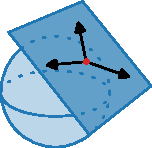
\includegraphics{figures/diagrams/tangent_space_sphere.pdf}
	\caption{The tangent space of the point \(\icon{figures/diagrams/dot_red.pdf}\in \c{S}_2\) with example tangent vectors.}
\end{figure}

\subsection{The differential}

If we have a smooth function between manifolds \(F: X\to Y\), we can also define a natural map between their tangent spaces at a point \(p\in X\) and \(F(p)\in Y\).
We call this the \emphmarginnote{differential} of \(F\) at \(p\), denoted \(\d F: T_pX\to T_{F(p)}Y\), and it is defined by its action on a tangent vector \(v \in T_pX\) and a smooth function on \(Y\), \(f\in C^\infty (Y)\).
\[\sbr{\d F_p (v)}\del{f} = v \del{f \circ F}(p), \quad v\in T_pM, \; f\in C^\infty(Y) \].
This is a \emph{linear} map that distributes over compositions of maps between manifolds, \(\d_p\del{F\circ G} = \d F_{G(p)} \circ \d G_p\), and preserves the identity map, \(\d(\id_X)_p = \id_{T_pX}\).
Importantly if \(F\) is a \emph{diffeomorphism}, then \(\d F\) is an \emph{isomorphism} between tangent spaces and \(\del{\d F}^{-1} = \d \del{F^{-1}}\).

It is worth thinking about what the differential means intuitivly.
It says that if we have a smooth function \(f\) on \(Y\), we can take a derivation of this with respect to tangent vector  \(v\in T_pX\) by first transporting the function \(f\) from \(Y\) to \(X\) via \(F\), and then take the derivation of this new function with \(v\).

Sometimes the differntial is refered to as the \emphmarginnote{pushforward} of a tangent vector by \(F\), and is denoted
\[(F_*)_p: T_p X \to T_p Y\]

\begin{figure}[h]
	\documentclass[tikz,10pt]{standalone}
\usepackage[standalone,commands]{../../MJH}

\graphicspath{/Users/mhutchin/Documents/thesis/figures/diagrams/}

% \usepackage{tikz}
% \usetikzlibrary{positioning}

\usepackage{pgfplots}
\pgfplotsset{compat=1.17}
% \usepgfplotslibrary{external}
% \usepgfplotslibrary{groupplots}
% \usepgfplotslibrary{fillbetween}
% \usetikzlibrary{fadings}

\begin{document}
    % \tikzsetnextfilename{generative_model}
    \begin{tikzpicture}
        \node (simple) at (0,0) {
\includegraphics{/Users/mhutchin/Documents/thesis/figures/diagrams/differential.pdf}};
        \node (math) at (-3.3,-0.85) {\(X\)};
        \node (math) at (3.3,-0.7) {\(Y\)};
        \node (math) at (-.7,-1.3) {\(F\)};
        \node (math) at (-.7,.8) {\(\d F_p\)};
        \node (math) at (-2.3,.8) {\(v\)};
        \node (math) at (1.3,0.85) {\(\d F_p (v)\)};
        \node (math) at (-2.6,.2) {\(p\)};
        \node (math) at (1.2,.05) {\(F(p)\)};
    \end{tikzpicture}
\end{document}
	\caption{A smooth map between smooth manifolds \(F: X \to Y\) induces a natural map between the tangent spaces of \(p\) and \(F(p)\), the differential \(\d F_p\).}
\end{figure}

\subsection{Submersions, immersions and embeddings}

The definition of the differential allows us to classify smooth maps between manifolds.
If we have a map \(F: X\to Y\), at any point we can define the \emphmarginnote{rank of a map} \(F\) at a point \(p\in X\) to be the rank of the linear map \(\d F_p\).
This is the dimension of the image of the differential, \(\dim \im \d F_p \subseteq T_{F(p)}Y\).
The rank of a linear map is bounded by the minimum of the dimensions of its domain and codomain, so \(\rank F_p \leq \min \cbr{\dim X, \dim Y}\).
If \(F\) has the same rank everywhere, it is said to be of constant rank, \(\rank F\).

A \emphmarginnote{smooth submersion} is a smooth map \(F:X\to Y\) with \(\rank F = \dim Y\).
The simplest example of this is the Euclidean projection onto a subset of coordinates, \(F:\R^{m+n} \to \R^m\), \(F: (x_1, ..., x_{m+n}) \mapsto (x_1, ..., x_m)\).
A \emphmarginnote{smooth immersion} is a smooth map \(F:X\to Y\) with \(\rank F = \dim X\).
The simplest example of this is the Euclidean inclusion of coordinates, \(F:\R^{m} \to \R^{m+n}\), \(F: (x_1, ..., x_m) \mapsto (x_1, ..., x_{m+n})\).
Of most importance to us will be \emphmarginnote{smooth embeddings}.
These are smooth immersions \(F:X \to Y\) that are also \emph{topological embeddings}(\cref{sec:topo_subspaces}), an immersion that is a homeomorphism when inheriting the subspace topology in its image \(F(X) \subseteq Y\).

Smooth embeddings are particualrly useful when we can embed the manifold into Euclidean space.
This is useful from a techincial perspective as it allows us to transfer tools from the simplified setting of Euclidean space onto the surface of the manifold easily, and from a computational point of view as it allows us to respresent points on the surface of the manifold in a global way.
Instead of having to pick a collection of charts to cover the manifold and represent, we can pick a global (but slightly redundant) coordinate system.
In addition, from a deep learning perspective, embeddings make it much easier to define smooth maps between manifolds.
Again if we were to use charts, we would need to pick more than one to cover most manifolds, and as such we would need to ensure that the function we define (usually a learable function) smoothly agrees on the overlap of the charts.
With a pair of embeddings for the input and output manifolds into Euclidean space, we can instead define a single smmoth function from Euclidean space to Euclidean space and restrict its inputs and outputs to the embedded manifolds.

A question then remains, can we always embed a smmooth manifold smoothly into Euclidean space?
The answer is yes.
\begin{theorem}[Whitney Embedding Theorem]
	Every smooth \(n\) dimension smooth manifold (with or without boundary) admits a proper smooth embedding into \(\R^{2n+1}\).
\end{theorem}
\begin{proof}
	\textcite[Theorem 6.15]{lee2013smooth}
\end{proof}
Note the \emph{proper} part of this definition additionally restricts the preimage of compact sets under the embedding to also be compact.

\subsection{Local coordinates}

The concepts of tangent vectors and differentials just introduced are very abstract.
To understand them better, and make them computationally useful, we can introduce the concept of \emphmarginnote{coordinate vectors} to produce a basis on tangent spaces.

For the special case of \(\R^n\), we already know how to define a basis on the tangent space at \(p\in \R^n\), \(T_p\R^n\).
We simply take the partial differentials with respect to each input at the given point, \(\eval{\pd{}{x_1}}_p, .
.., \eval{\pd{}{x_n}}_p\).
Any derivation can then be expressed as \[v = \sum_{i=1}^n v^i \eval{\pd{}{x_i}}_p \quad\quad v \in T_p\R^n ,\; v_i \in \R\].
Their action on a smooth function \(f\in C^\infty(\R^n)\) is simply \[\eval{\pd{}{x_i}}_p \del{f} = \pd{f}{x_i}\del{p}\] 

Using this basis on \(T_p\R^n\), we can place a basis on a tangent space of a manifold \(T_pX\) at point using a smooth chart \((U, \phi)\in \atlas{X}\) containing that point.
Remember that a smooth chart \(\phi: U \to \R^n\) is a diffeomorphism onto its image.
Therefore, the differential \(\d \phi_p: T_pX \to T_{\phi(p)}\R^n\) is an isomorphism.
We can define a basis on \(T_pX\) then as the \emph{preimage} of the standard basis on \(T_{\phi(p)}\R^n\) under \(\phi\).
Let us then define the basis vector \[\eval{\pd{}{\phi_i}}_{ p} = \del{\d \phi_p}^{-1} \del{\eval{\pd{}{x_i}}_{\phi({p})}} = d\del{\phi^{-1}}_{\phi(p)}\del{\eval{\pd{}{x_i}}_{\phi({p})}}\].
Often, \(\eval{\pd{}{\phi_i}}_{p}\) is denoted as \(\eval{\pd{}{x_i}}_{p}\), obscuring the dependence on \(\phi\) and potentially confusing it with the basis vector of \(T_{\phi(p)}\R^n\) that it is related to, \( \eval{\pd{}{x_i}}_{\phi(p)}\).
For further simplicity, the notation is often shortened further to \[\eval{\pd{}{\phi_i}}_{p} = \eval{\partial \phi_i}_p = \eval{\partial x_i}_p = \eval{\partial_i}_p\] when the chart and local coordinates are implied.
The action of one of these basis vectors on a function \(f\in C^\infty(X)\) is then \[\eval{\pd{}{\phi_i}}_{p}f = \eval{\pd{}{x_i}}_{\phi(p)} \del{f \circ \phi^{-1}}\].
We can then express any tangent vector \(v \in T_pX\) as \[v = \sum_{i=1}^n v_i \eval{\pd{}{\phi_i}}_p \quad\quad v \in T_pX ,\; v_i \in \R \] \begin{figure}[h] \documentclass[tikz,10pt]{standalone}
\usepackage[standalone,commands]{../../MJH}

\graphicspath{/home/mhutchin/GoogleDrive/University - Postgraduate/Theses/Final/figures/diagrams/}

% \usepackage{tikz}
% \usetikzlibrary{positioning}

\usepackage{pgfplots}
\pgfplotsset{compat=1.17}
% \usepgfplotslibrary{external}
% \usepgfplotslibrary{groupplots}
% \usepgfplotslibrary{fillbetween}
% \usetikzlibrary{fadings}

\begin{document}
    % \tikzsetnextfilename{generative_model}
    \begin{tikzpicture}
        \node (simple) at (0,0) {
\includegraphics{/home/mhutchin/GoogleDrive/University - Postgraduate/Theses/Final/figures/diagrams/tangent_basis.pdf}};
        \node (math) at (-4.5,-0.3) {\(U \subset X\)};
        \node (math) at (-1.8,-1.7) {\(\phi\)};
        \node (math) at (-1.4,-0.75) {\(\d \phi_p\)};
        \node (math) at (4.5,-1.) {\(Y \subset \R^n\)};
        \node (math) at (1.4,0.1) {\(T_{\phi(p)}\R^n\)};
        \node (math) at (-3.8,1.1) {\(T_{p}X\)};
        \node (math) at (-3.1,.4) {\(p\)};
        \node (math) at (0.1,.8) {\(\phi(p)\)};
        \node (math) at (-2.,.6) {\(\eval{\partial\phi_\text{lon}}_{p}\)};
        \node (math) at (-2.9,1.3) {\(\eval{\partial\phi_\text{lat}}_{p}\)};
        \node (math) at (1.85,.85) {\(\eval{\partial x_\text{lon}}_{\phi(p)}\)};
        \node (math) at (1.2,1.4) {\(\eval{\partial x_\text{lat}}_{\phi(p)}\)};
        \node (math) at (4.7,0.05) {\(x_\text{lon}\)};
        \node (math) at (3.3,1.4) {\(x_\text{lat}\)};
        % \node (math) at (1.2,.05) {\(F(p)\)};



        % \node (math2) at (-1.5,-1) {\(V\)};

        % \node (math2) at (-1.6,-0.2) {\(U \u V\)};

        % \node (math) at (-0,1.0) {\(\phi_U\)};
        % \node (math) at (-0,-0.7) {\(\phi_V\)};

        % \node (math) at (2.5,0) {\(\phi_V \circ \phi^{-1}_U\)};


        % \node (complex) at (3,0) {
\includegraphics{../diagrams/simple_distribution.pdf}};
        % \draw[-stealth] (math.north) to [out=45,in=135] (math2.north) node [midway, yshift=1.1cm] {\(f\)} ;
        % \draw[-stealth] (math2.west) to (math.east) node [midway, above] {\(f^{-1}(V) = U\)} ;
    \end{tikzpicture}
\end{document} \caption{Using a chart on the sphere that maps from points on the sphere to their latitude and longitude, we can induce a basis on the tangent space on the sphere in the latitude and longitude direction via the differential of the chart.
	}
\end{figure}
\begin{figure}[h]
	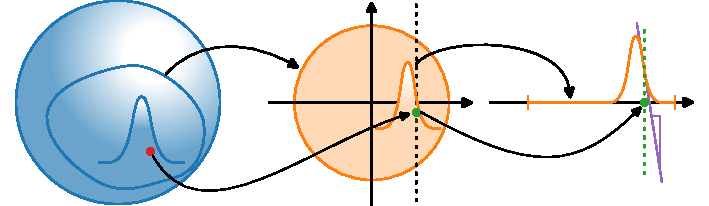
\includegraphics{figures/diagrams/coordinate_differential.pdf}
	\caption{Taking the differential of \(f\), a bump function, evaluated at \(p\) in the i'th direction.
		Push the function \(f\) onto the chart \(U\) through \(\phi\) to give the function \(f\circ \phi^{-1}: \R^k\to \R\).
		Then restrict this function to the i'th component to give \(\eval{f\circ \phi^{-1}}_i: \R \to \R\).
		Finally, evaluate the derivative of this as usual, in purple here at the i'th coordinate of \(\phi(p)\).
	}
\end{figure}

We can also study how the \emphmarginnote{differential in local coordinates} looks.
First again let us consider the special case of \(F: U\subseteq\R^n \to V\subseteq\R^m\), with the standard basis for the tangent spaces \(\eval{\pd{}{x_1}}_p, .
.., \eval{\pd{}{x_n}}_p\) and \(\eval{\pd{}{y_1}}_q, ..., \eval{\pd{}{y_m}}_q\).
Applying the definition of the differential and the chain rule to a function \(f\in C^\infty (\R^m)\), we get \[\d F_p\del{\eval{\pd{}{x_i}}_p}f &= \eval{\pd{}{x_i}}_p \del{f \circ F}\nonumber \\ &= \sum_{j=1}^m \pd{f}{y_j}\del{F(p)} \pd{F_j}{x_i}(p) \nonumber \\ &= \del{\sum_{j=1}^m \pd{F_j}{x_i}(p) \eval{\pd{}{y_j}}_{F(p)}} f\].
Therefore, \[\d F_p\del{\eval{\pd{}{x_i}}_p} = \sum_{j=1}^m \pd{F_j}{x_i}(p) \eval{\pd{}{y_j}}_{F(p)} \].
If we have \(v = \sum_{i=1}^n v_i \eval{\pd{}{x_i}}_p\), then its image under the differential, \(w = \d F(v)\) in basis coefficients is \[\begin{bmatrix} w_1 \\ \vdots \\ w_m \end{bmatrix} = \begin{bmatrix} \pd{F_1}{x_1}(p) & \dots & \pd{F_1}{x_n}(p) \\ \vdots & \ddots & \vdots \\ \pd{F_m}{x_1}(p) & \dots & \pd{F_m}{x_n}(p) \end{bmatrix}\begin{bmatrix} v_1 \\ \vdots \\ v_n \end{bmatrix}\].
So we see in local coordinates the differential is associated with a matrix with entries \(\pd{F_j}{x_i}\).
This is exactly the \emphmarginnote{Jacobian matrix} of \(F\).
The differential is therefore the coordinate-free definition of the Jacobian.

In order to apply this to the differential of \(F: X \to Y\), we again look at the behaviour with respect to charts.
Pick two charts \((U, \phi)\in \atlas{X}\), \(p\in U\), and \((V, \psi)\in \atlas{Y}\), \(F(p)\in V\), and write that \(\tilde{F} = \psi \circ F \circ \phi^{-1}\), so \( F = \psi^{-1} \circ \tilde F \circ \phi\).
We know that \(\d \tilde F _{\phi(p)}\) in coordinates is the matrix described above, \(\pd{\tilde F_j}{x_i}\).
We can then write \[\d F_p \del{\eval{\pd{}{\phi_i}}_p} = \d \del{\psi^{-1} \circ \tilde F \circ \phi}_p \del{\eval{\pd{}{\phi_i}}_p} &= \d {\psi^{-1}}_{F(p)} \circ \d {\tilde F}_{\phi(p)} \circ \d {\phi}_p \del{\eval{\pd{}{\phi_i}}_p} \\&= \d {\psi^{-1}}_{F(p)} \circ \d {\tilde F}_{\phi(p)} \del{\eval{\pd{}{x_i}}_{\phi(p)}} \\ &= \d {\psi^{-1}}_{F(p)} \del{\sum_{j=1}^m \pd{\tilde F_j}{x_i}\eval{\pd{}{y_j}}_{\psi(p)}} \\ &= \sum_{j=1}^m \pd{\tilde F_j}{x_i}\eval{\pd{}{\psi_j}}_{p}\].
So again we see that the differential is associated in local coordinates with the Jacobian matrix \(\pd{\tilde F_j}{x_i}\).
The rank of this Jacobian matrix in the usual matrix sense is equal to the more abstract rank of the differential, \(\dim \im \d F_p \subseteq T_{F(p)}N\).

One particular example of the differential in coordinates is in the effect on tangent vectors under a change in chart, called a \emphmarginnote{change in coordinate}.
If we have \(p\) in two charts \((U, \phi)\), \((V, \psi)\) and a vector \(v\) at \(p\), in the two different chart bases, \(v = \sum_{i=1}^n a_i \eval{\pd{}{\phi_i}}_p = \sum_{i=1}^n b_i \eval{\pd{}{\psi_i}}_p\), then the basis coefficients are related by \(b_j = \sum_{i=1}^n \pd{\psi \circ \phi^{-1}_j}{x_i} a_i\).
As a small abuse of notation I will write \(\pd{\psi \circ \phi^{-1}_j}{x_i} = \pd{\psi_j}{\phi_i}\).

Since we know this differential is an isomorphism, so must its Jacobian, i.e. is it full rank, so \(\pd{\psi_j}{\phi_i}\in \groupGL\).
This group that related the basis coefficients of different bases of the tangent space is called the \emphmarginnote{structure group} of the manifold.
If we have additional structure on our manifold, we can get a \emphmarginnote{reduced structure group} \(G\subset \groupGL\) by preferring a subset of specific bases on each tangent space.
\todo{talk more on structure groups, frame bundles etc?
	COvered well by weiler.
}.
For example, if we have a notion of an inner product on the tangent space, we can prefer orthonormal bases and reduce the structure group to \(\groupO\).
If our manifold is \emph{orientable} then we can 

\begin{figure}[h] 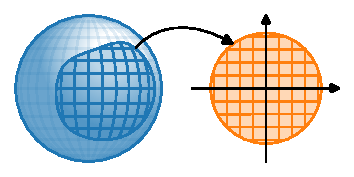
\includegraphics{figures/diagrams/coordinate_chart.pdf} \caption{A coordinate chart of the sphere, \(\c{S}_2\).
	}
\end{figure}

\begin{figure}[h]
	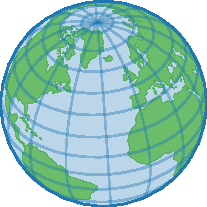
\includegraphics{figures/diagrams/earth.pdf}
\end{figure}

\subsection{Cotangent and tensor spaces}

On a manifold, we denote the \emphmarginnote{cotangent space} at \(p\), \(T^*_pX\) to be the dual of the tangent space \[T^*_pX = \del{T_pX}^*\].
Elements of this are called \emphmarginnote{cotangent vectors}.

With the tangent space and cotangent space defined at a point \(p\), we can define also define the \emphmarginnote{tensor space} \((T_s^r)_pX\) as
\[(T_s^r)_pX = T_s^r(T_pX) = \underbrace{T_pX\otimes ... \otimes T_pX}_{r\text{ copies}} \otimes \underbrace{T_pX^*\otimes ... \otimes T_pX^*}_{s\text{ copies}} \]

Given a chart on the manifold, \((U, \phi)\), and the induced basis on the tangent space, \(\cbr{\eval{\partial \phi_i}_p}\), we can define a basis on the cotangent space, \(\cbr{\eval{\d\phi^{i}}_p}\) by \(\eval{\d\phi^i}_p (\eval{\partial \phi_j}_p) = \delta^i_j\).
% Our choice of notation of \(\eval{\d \phi_i}_p\) will become apparent.

Previously, we saw how under a change of coordinates from \((U, \phi)\) to \((V, \psi)\) the coefficients of a tangent vector \(v\in T_pX\) transformed under the Jacobian of the differential.
The coefficients of a cotangent vector also transform under the Jacobian, but in the opposite way.
For \(v\in T_pX\), \(v = v^i \eval{\partial\phi_i}_p = \tilde v^i \eval{\partial \psi_i}_p\) and \(\omega \in T^*_pX\), \(\omega = \omega_i \eval{\d\phi_i}_p = \tilde \omega_i \eval{\d\psi_i}_p\) we get the transforms \[\underset{\text{Tangent vector transformation}}{\tilde v^j = \pd{\psi^j}{\phi^i}(p) v^i} \quad \quad \quad \underset{\text{Cotangent vector transformation}}{\omega_i = \pd{\psi^j}{\phi^i}(p)\tilde \omega_j}\].
This transform definition is equivalent to saying that \(\tilde \omega_j = \del{\pd{\psi^j}{\phi^i}(p)}^{-1} \omega_i\).
Plugging this into the definition of the cotangent vectors and working it through in coordinates, we see that this leave the action of the cotangent vector on the tangent vector in coordinates invariant to the choice of coordinates, as we would expect.

Previously we saw the defintion of the \emph{pushforward} of a tangent vector along a diffeomporphism \(F: X\to Y\) from \(T_pX\) to \(T_pY\).
We can instead \emphmarginnote{pullback} a covector from \(T_pY^*\) to \(T_pX^*\) via the pullback \((F^*)_p: T_pY^*\to T_pX^*\), defined by its action on a vector \(v\in T_pX\),
\[((F^*)_p(\omega))(v) = \omega((F_*)_p(v))\]

\section{Tensor Bundles}

\subsection{Tangent bundles and vector fields}

We have just considered the tangent space of a point \(p\) on a manifold \(X\).
What if we want to consider the tangent space at every point on a manifold simultaneously?
This leads us to the notion of the tangent \emph{bundle}.

We construct the \emphmarginnote{tangent bundle} by taking the set \emph{disjoint union} of the tangent spaces, \[TX = \disjointU_{p\in X} T_pX = \cbrcolon{(x, v)}{x\in X, v\in T_xX}\].
Along with this we have a \emphmarginnote{canonical projection} \(\pi : TX \to X\), defined by \(\pi: (x, v) \mapsto x\).
The topology we place on this is \emph{not} however the disjoint union topology.
The disjoint union topology would leave each tangent space topologically disconnected from each other.
Instead, we give it a \emphmarginnote{natural topology} that renders the tangent bundle itself also a manifold of dimension \(2n\).

\begin{proposition}[The tangent bundle is a smooth manifold]
	For any smooth \(n\)-dimension manifold \(X\), the tangent bundle is a \(2n\)-dimension smooth manifold with a natural topology and smooth structure.
	With respect to this structure, the projection \(\pi: TX \to X\) is smooth.
\end{proposition} 

\begin{proof} To do this, we construct charts that satisfy the smooth chart lemma (\cref{lem:smooth_chart}).

	We construct our charts on \(TX\) out of the atlas of the base manifold \(\atlas{X}\).

	Take any chart in \(\atlas{X}\), \((U, \phi)\).
	We construct a new chart \(\Phi: TU \to \R^{2n}\) (\(TU = \coprod_{p\in U} T_pX\)) by taking the coordinate functions \(\phi_i: U \to \R\) and the induced basis on the tangent space \(T_pX\), \(\eval{\partial \phi_i}_p\).
	Defining \[\Phi(p, v^i\eval{\partial \phi_i}_p) = \del{\phi_1(p), .
			.., \phi_n(p), v_1, ..., v_n}\].
	This is a bijection as its inverse is \[\Phi^{-1}(x_1, .
		.., x_n, v_1, ..., v_n) = \del{\phi^{-1}(x_1, ..., x_n), v^i\eval{\phi_i}_{\phi^{-1}(x_1, ..., x_n)}}\].
	For \(\Psi\) constructed similarly to \(\Phi\), the transition function \(\Psi \circ \Phi^{-1}\) is given by \[\Psi \circ \Phi^{-1}(x_1, .
		.., x_n, v_1, ..., v_n) = \del{\del{\psi\circ\phi^{-1}}(x_1, ..., x_n), \sum_{i=1}^n \pd{\psi_1}{\phi_i} v_i, ..., \sum_{i=1}^n \pd{\psi_n}{\phi_i}v_i} \] which is smooth.

	To satisfy the smooth chart lemma: \begin{enumerate}[noitemsep] \item For any chart \((TU, \Phi)\), this is a bijection onto \(\phi(U)\x \R^n \underset{\text{open}}{\subseteq} \R^n \x \R^n\), an open set of \(\R^{2n}\).
		\item Similarly, for \((TU, \Phi)\), \((TV, \Psi)\), \(\Phi(TU\^TV)\) and \(\Psi(TU\^TV)\) are open subsets of \(\R^n\).
		\item The transition maps \(\Psi \circ \Phi^{-1}\) are smooth as shown.
		\item We can pick a countable cover of \(TX\) by taking a countable cover of \(X\) and use those charts to construct our charts on \(TX\).
		\item If we have \((p,v_1), (p, v_2)\) and a set \(p \in U\), then \((p,v_1), (p, v_2) \in TU\).
		      If we have \((p,v), (q, w)\), \(p\neq q\), then from the charts of \(X\) we have \(U, V\) such that they are disjoint and \(p\in U\), \(q \in V\).
		      Therefore \((p, v)\in TU\), and \((q, w)\in TV\), but \(TU, TV\) are disjoint.
	\end{enumerate}

	To show that \(\pi\) is smooth, note that \(\pi: (x, v) \mapsto x\).
	In charts \((U, \phi)\), \((TU, \Phi)\) this is simply a restriction to the first half of the coordinates, with is smooth.
\end{proof}

This object we have constructed is an example of a fibre bundle introduced earlier (\cref{def:fibre_bundle}), as the triple \((TX, \pi, X)\).

The sections of the tangent bundle are called \emphmarginnote{vector fields}.
In the Euclidean setting, this amounts to continuous map from \(\R^n \to \R^n\) (or open subsets of), that can be visualised as an "arrow" at each point.
In the sense of the direction derivative discussed earlier, this akin to attaching a directional derivative to each point.
A \emphmarginnote{vector field on a smooth manifold} is then a section of the tangent bundle instead.

A \emphmarginnote{smooth vector field} is one that is a smooth function between \(X\) and \(TX\).
A \emphmarginnote[\baselineskip]{rough vector field} is one that is not.

We will denote the space of vector fields as \(\Gamma(TX)\).
Sometimes it is written as \(\mathfrak{X}(X)\).

\subsubsection{Algebraic structure of the tangent bundle}
In the previous section we saw that tanget spaces \emph{at a point} can be viewed as a specific algebraic structure, namely as the \emph{vector space} of \emph{derivations at a point} over the \emph{algebra} of smooth functions \((C^\infty(X), +, \cdot, \bullet)\). 
% Recall that we set \(+\) to be pointwise addition of functions, \(\cdot\) to be pointwise multiplication of functions, and \(\bullet\) to be multiplication of the function by a scalar.
Recall that we had:
\begin{itemize}
	\item \(+: C^\infty(X)\times C^\infty(X) \to C^\infty(X)\) to be pointwise addition of functions.
	\item \(\cdot: \R \times C^\infty(X) \to C^\infty(X) \) to be pointwise multiplication by a scalar.
	\item \(\bullet:C^\infty(X)\times C^\infty(X) \to C^\infty(X) \) to be pointwise multiplication of functions.
\end{itemize}
Lets then define:
\begin{itemize}
	\item \(\oplus: \Gamma(TX)\times \Gamma(TX)\to \Gamma(TX)\), \((\sigma\oplus \tau)(p) \mapsto \sigma(p) + \tau(p)\), pointwise vector addition of vector fields.
	\item \(\odot: C^\infty(X) \times \Gamma(TX) \to \Gamma(TX)\), \((f\odot \sigma)(p) \mapsto f(p)\sigma(p)\), pointwise scaling of a vector field by a function.
\end{itemize}

We can construct a \emph{ring} (\cref{def:ring}) from the smooth functions on a manifold as \((C^\infty(X), +, \bullet)\).
The triple \((\Gamma(TX), \oplus, \odot)\) then satisfies the conditions of a \emph{vector space} with respect to this \emph{ring}.
Vector spaces over rings are very different to vector spaces over fields, and are often called \emphmarginnote{modules}.

It is possible to define \(\Gamma(TX)\) as a vector space over the field \(\R\) by using \emph{global} scaling of a vector field by a constant, but the \emph{basis} of this vector space nessicarily becomes uncountably infinite and difficult to work with.
By contrast \(\Gamma(TX)\) as a vector space over the ring \(C^\infty(X)\) by using \emph{local} scaling of a vector field by a function is more natural and plesant to work with.
See \cite{schuller2013lectures}. \todo{module theory?}

As a summary:\\
\(T_pX\) is a \emph{vector space} over the \emph{field \(\R\)} of \emph{derivations at a point} of the \emph{algebra} \(C^\infty(X)\).\\
\(\Gamma(TX)\) is a \emph{vector space} over the \emph{ring \(C^\infty(X)\)} of \emph{derivations} of the \emph{algebra} \(C^\infty(X)\).

This algebric description of the space of vector fields in fact is an alternative way to define the space, in lieu of the previoulsy presented construction.

\subsubsection{Local bases for vector fields}

We can write a vector field using its \emphmarginnote{component functions} at a given point using the basis vectors induced by a chart \((U, \phi)\), \[V_p = \sum_{i=1}^n V_i(p) \eval{\pd{}{\phi_i}}_p\].
This defines the component function \(V_i(p) : U \to \R\).
A vector field is smooth if and only if its component functions in each chart are smooth.

A chart induces \emphmarginnote{coordinate vector fields} on \(U\subseteq X\) by the assignment \(p\mapsto \eval{\pd{}{\phi_i}}_p\).
These are denoted as \(\pd{}{\phi_i} = \partial\phi_i = \partial_i\) where the rest of the information is implicit.
Together, the coordinate vector fields \(\partial\phi_1, .
.. \partial \phi_n\) produce a \emph{smooth local frame} called a \emphmarginnote{coordinate frame}.
A \emphmarginnote{smooth local frame} a set of smooth (restricted to an open set \(U\)) vector fields that at each point span the tangent space.
If \(U=X\), this is a global frame, although these do not exist for most manifolds \todo{say something more?
}.

An important operation we can perform on vector fields is the \emphmarginnote{Lie bracket}.
For \(V, W \in \Gamma(TX)\), we define the operation \(\sbr{V, W}: \C^\infty(X)\to C^\infty(X)\) as \[ \sbr{V, W}f = V(Wf) - W(Vf)\].
This has a number of properties.
For \(U,V,W \in \Gamma\del{TX}\) we have \begin{enumerate}[noitemsep] \item \(\sbr{V,W}\) is bilinear.
	\item \(\sbr{V, W} = -\sbr{W,V}\), it is antisymmetric.
	\item \(\sbr{U,\sbr{V, W}} + \sbr{W,\sbr{U, V}} + \sbr{V,\sbr{W, U}} = 0\), the Jacobi identity.
	\item For \(f, g\in C^\infty(X)\), \(\sbr{fV, gW} = fg\sbr{V,W} + f(Vg)W - (gWf)V\), relating the two ways of actioning smooth functions and vector fields.
\end{enumerate}
\todo{why is this important?}

\subsection{Tesor bundles and fields}
The tangent bundle is one of the most fundamental bundles we deal with in geometry.
We can however introduce a wider range of bundles by bundling arbitray tensors over the manifold (\cref{sec:higher_order_tensors}).
All of these bundles will be examples of \emph{vector bundles}, which are fibre bundles where the typical fibre is isomorphic to \(\R^n\) with the usual vector structure.

In constructing these bundles, it is very handy to have the following lemma.
\begin{lemma}[Vector bundle chart lemma]
	Let \(X\) be a smooth manifold (with boundary), and suppose that for each \(p\in X\) we have \(E_p\), a \(k\)-dimension vector space.
	Let \(E = \coprod_{p\in X} E_p\), and \(\pi: E\to X\) be the map such that \(\pi: E_p \mapsto p\).
	If have the following: \begin{enumerate}[noitemsep] \item an open cover of \(X\), \(\cbr{U_a}_{a\in A}\).
		\item for each \(a \in A\), a bijection \(\Phi: \pi^{-1}(U_a) \to U_a \times \R^k\).
		\item for each \(a, b\in A\) with \(U_a \^ U_b \neq \emptyset\), a smooth map \(\tau_{ab}
		      U_a\^ U_b \to \groupGL[k, \R]\) such that the map \(\Phi_a\circ \Phi_b^{-1}: (U_a\^ U_b) \times \R^k \to (U_a\^ U_b) \times \R^k\) is of the form \[ \Phi_a\circ \Phi_b^{-1}(p, v) = (p, \tau_{ab}(p)v)\] \end{enumerate} Then E has a unique topology and smooth structure making it into a smooth manifold with or without boundary and a smooth rank-k vector bundle over M; with \(\pi\) as projection and \(\cbr{(U_a, \Phi_a)}\) as smooth local trivializations.
\end{lemma}
Using this we could have constructed the target bundle by creating the transition maps as we did, and applying this lemma.

Identically to the tangent bundle then, we can build the \emphmarginnote{cotangent bundle}, denoted by \(T^*X\), from cotangent spaces. 
This too is a \(2n\)-dimension manifold and a vector bundle.
We build the natural coordinates again out of the basis induced by charts, in this case from the dual basis of the tangent basis. 
Sections of this are called \emphmarginnote{covector fields}, denoted \(\omega \in \Gamma(T^*X)\).
The action of a covector field \(\omega \in \Gamma{T^*X}\) on a vector field \(V \in \Gamma(TX)\) is defined by \[\omega(V): X \to \R, \quad\quad \omega(V)(p) = \omega_p(V_p)\].

More generally we can bundle tensor spaces at every point to give \emphmarginnote{tensor bundles}, denoted by \(T^p_qTX\).
We gain construct this using the vector bundle chart lemma, and use a basis everywhere from the basis of the tangent bundle and cotangent bundle, the same as in \cref{sec:vector_bases}.

There are a series of special cases.\\
The \emph{tangent bundle} is denoted \(TX = T^1_0TX\)\\
The \emph{cotangent bundle} is denoted \(T^*X = T^0_1TX\)\\
The \emphmarginnote{bundle of covariant \(k\)-tensors} is denoted \(T^kT^*X = T^0_kTX\).\\
The \emphmarginnote{bundle of contravariant \(k\)-tensors} is denoted \(T^kTX = T^k_0TX\).\\
The \emphmarginnote{bundle of symmetric \(k\)-tensors} is denoted \(\Sigma^kT^*X = \sym T^0_kTX\).\\
The \emphmarginnote{bundle of alternating \(k\)-tensors} is denoted \(\Lambda^kT^*X = \alt T^0_kTX\).

A \emphmarginnote{tensor field} is then a \emph{smooth section} of a tensor bundle.
The space of smooth sections of a tensor bundle is denoted \(\Gamma\del{T^p_qT}\).
\(\Gamma\del{T^0_0TX}\) is simply the space of smooth functions \(C^\infty(X)\).

\subsusbection{Bases for sections of tensor bundles}

For tensor bundles we can again define smooth local \emph{frames}.
If we have a smooth local frame for the tangent bundle \(e_1, ..., e_n\), then we can define the local \emphmarginnote{dual coframe} as the vector fields \(\epsilon^1, ..., \epsilon^n\) such that \(\epsilon^i(e_j) = \delta^i_j\).
If we have a chart \((\phi, U)\) and therefore tangent frames \(\partial \phi_i\), then the dual frames are the differenitals of the chart, \(\d\phi_i\).
From this we can construct smooth local frames on any tensor bundle in terms of a local frame of the tangent bundle. 
For a \(T^p_q TX\) bundle, the smooth local frames are given by 
\[
	e_{i_1} \otimes ...\otimes e_{i_p} \otimes \epsilon^{j_1} \otimes ... \otimes \epsilon^{j_q}	
\].
For a given char t \((U, \phi)\), a tensor field \(F\) can be expressed locally as
\[
	F = F_{j_1, ..., j_q}^{i_1, ..., i_p} \partial\phi_{i_1} \otimes ...\otimes \partial\phi_{i_p} \otimes \d\phi^{j_1} \otimes ... \otimes \d\phi^{j_q}	
\]
where the \(F_{j_1, ..., j_q}^{i_1, ..., i_p}: U \to \R\) are smooth functions.

One of the most important intepretations of tensor fields is as \emphmarginnote{smooth multilinear maps over \(C^\infty(X)\)}.
For a \(T^p_qTX\) tensor field \(F\in \Gamma\del{T^p_qTX}\), this can be seen as the map
\[F: \underbrace{T^*X \times ... \times T^*m}_{p\text{ \emph{covector} fields}}\times\underbrace{TX \times ... \times Tm}_{p\text{ \emph{vector} fields}} \to C^\infty(X)\].
This map is smooth, and multilinear. 
In fact, all smooth multilinear maps of this form are induced by tensor fields (\cref[Lemma 12.24 extends naturall to mixed tensor fields]{lee2013smooth}).

\subsubsection{Algebraic structure of tensor bundles}
\todo{module structuressss}
can do the multilinear maps this way

\subsubsection{Pullbacks of tensor fields}

Previously we say how using the differential we could pushforward and pullback tangent and cotangent vectors between the tangent spaces of two manifolds related by a smooth function \(F:X\to Y\).
We can define the \emphmarginnote{pullback of a covaraint tensor field} pointwise.
For \(A \in \Gamma(T^kT^*Y)\), the \emph{pointwise pullback} of \(\d F(A) \in \Gamma(T^kT^*X)\) is given by
\[[\d F ^*(A)]_p(v_1, ..., v_n) = A_p(\d F_p (v_1), ..., \d F_p (v_k))\]
for \(v_1, ..., v_k \in \Gamma(TX)\).

\section{Differential Forms and integration}


\section{Orientations}
\section{Line Integrals}
\section{Integration on Manifolds}


\section{Riemannian Metrics}
We now turn our study to \emph{Riemannian} manifolds. 
So far we have defined manifolds with notions of topology, smoothness and differentation. 
However we are yet to introduce geometry, in simple terms the studay of lengths and angles.
In metic spaces such ideas are studied through the direct definition of a metric.
On manifolds however the more natural object to study these concepts through is a \emph{Riemannian metric}.

For the rest of this section, we assume that \(X\) is a smooth manifold with or without boundary.

\subsection{Riemannian metrics}
The most important concept to transfer from Euclidean space is the notion of lengths of vectors, and inner products between vectors.

\begin{definition}[Riemannian metric]
	A \emph{Riemannian metric} \(g\) is a smooth section of the symmetric covariant 2-tensor field on \(X\).
	That is,
	\[g\in \Sigma^2 TX \]
\end{definition}
\begin{definition}[Riemannain manifold]
	A \emph{Riemannian manifold} (with or without boundary) \((X, g)\) is a smooth manifold (with or without boundary) \(X\) along with a Riemannain metric \(g\in \Sigma^2 TX\).
\end{definition}
It should be noted a Riemannian metric is \emph{not} the same as a metric in the metric space sens,e and we will distinguish these by calling them \emphmarginnote{distance functions}.

By looking at the metric restricted to a particualr point on the manifold, \(g_p: T_pX\times T_pX \to \R\), we see that this defines an inner product on the tangent space, as the metric is a symmetric tensor and therefore \(g_p(v, v) \geq 0\) for \(v \in T_pX\).

We can express the metric in the coordinates of a chart \((U, \phi)\) as 
\[g = g_{ij}\d\phi^i \otimes \d\phi^j = g_{ij} \d\phi^i\d\phi^j\]

The simplest metric is the \emph{Euclidean metric},
\[g = \delta_{ij}\d\phi^i\d\phi^j = (\d\phi^i)^2\]
and from this we recover all the usual notations of Euclidean space.
In particular note that the inner product defined for two vectors \(v, w\in T_pX\) is given by
\[g_p(v, w) = \delta_{ij} v^i w^j = \sum_{i=1}^n v^i w^i\], the usual dot product.
Note how the last expression violates the index convention of einsum notation, nessecitating the use of explicit sums, revealing how the usual definition of the dot product leave some inaacuracy in geometric terms.
Often an alternative notation is used, \(g_p(v, w) = \innerprod{v}{w}_p\).

Every smooth manifold admits a metric \parencite[proposition 13.3]{lee2013smooth}.
Every smooth manifold admits a huge variety of metrics in fact, and as such there is no canonical choice of Riemanina metric. \todo{examples}

We can define the \emphmarginnote{product metric} on a product of Riemannian manifolds by applying each metric to the components of the tangent vectors that cam from each manifold in the product, and so define \emphmarginnote{product Riemannian manifolds}.

From the definition of a Riemannian metric, we can then define the \emphmarginnote{length} of a tanget vector as \[|v|_g = \innerprod{v}{v}_g^{1/2} = g_p(v, v)^{1/2}\], and the \emphmarginnote{angle between tangent vectors} as \[\cos \theta = \frac{\innerprod{v}{w}}{|v|_g|w|_g}\]. 
We can say that two tangent vectors are \emphmarginnote{orthonormal} if \(\innerprod{v}{w} = 0\).
An \emphmarginnote{orthonormal frame} on a manifold is a frame for which at each point on the manifold, the basis on the tangent space is comprised of vectors orthonormal to each other.
The existence of smooth \emphmarginnote{locally orthonormal frames} is guarenteed \parencite[corollary 13.8]{lee2013smooth}, but the existence of smooth \emphmarginnote{globally orthonormal frames} is not guarenteed, and in fact only exist for a very small class of manifolds, such as Euclidean space.

\subsection{Pullback metrics and submanifolds}

If we have a smooth map \(F: X\to Y\) and a Riemannian metric on \(Y\), then the \emphmarginnote{pullback of the Riemannian metric} \(F^*g\) is a Riemannian metric on \(X\) if and only if \(F\) is a smooth immersion \parencite[proposition 13.9]{lee2013smooth}.

If we have two Riemannian manifolds \((X, g)\) and \((\tilde X, \tilde g)\), and a diffeomorphism \(F: X\to \tilde X\), then \(F\) is a \emphmarginnote{Riemannian isometry} if \(F^*\tilde g = g\).
If there exists such an isometry between two manifolds, we say they are \emphmarginnote{isometric}.
If this property only holds locally for two manifolds, but not globally, then they are said to be \emphmarginnote{locally isometric}.
The study of properties that are invariant under global or local Riemannian isometries is called \emphmarginnote{Riemannian geometry}.
One such property of a manifold is if it is \emphmarginnote{flat}.
A manifold is flat if it is locally isometric to Euclidean space equipped with the Eucldiean metric.

The most useful case for us of pullback metrics is for inducing metrics on submanifolds.


\section{Lie Groups and Lie Algebras}
\section{Principle Bundles}

\section{Connections and Parallel Transport}
\section{Geodesics, Exponential and Logarithm Maps, Riemannian Distance functions}